\newpage
\section{ĐƯỜNG THẲNG VÀ MẶT PHẲNG SONG SONG}
\subsection{LÝ THUYẾT CẦN NHỚ}
\subsubsection{Vị trí tương đối giữa đường thẳng và mặt phẳng}
\begin{khung4}{}
Cho đường thẳng $a$ và mặt phẳng $(P)$. Khi đó có thể xảy ra một trong ba trường hợp sau
\begin{itemize}
	\item Trường hợp 1: $a$ và $(P)$ có từ hai điểm chung phân biệt trở lên (hình a), suy ra mọi điểm thuộc $a$ đều thuộc $(P)$, ta nói $a$ nằm trong $(P)$, kí hiệu $a\subset (P)$.
	\item Trường hợp 2: $a$ và $(P)$ có một điểm chung duy nhất $A$ (hình b), ta nói $a$ cắt $(P)$ tại $A$, kí hiệu $a\cap (P)=A$.
	\item Trường hợp 3: $a$ và $(P)$ không có điểm chung nào (hình c), ta nói $a$ song song với $(P)$, kí hiệu $a\parallel (P)$.
\end{itemize}
\begin{center}
	\begin{tikzpicture}[scale=1, font=\footnotesize, line join=round, line cap=round, >=stealth]
		\begin{scope}
			\path
			(0,0) coordinate (A)
			(4,0) coordinate (B)
			(1,2) coordinate (D)
			($(B)+(D)-(A)$) coordinate (C)
			(1,.6) coordinate (E)
			(4,1.5) coordinate (F)
			;
			\draw    pic["$P$", draw=black, angle eccentricity=.7, angle radius=1cm]
			{angle=B--A--D}; %góc
			\draw($(E)!0.9!(F)$)node[above]{$a$} (E)--(F) (A)--(B)--(C)--(D)--cycle;
			\node at ($(A)+(-35:2.3)$) {$\text{Hình a)}$};
		\end{scope}
		\begin{scope}[xshift=5.5cm]
			\path
			(0,0) coordinate (A)
			(4,0) coordinate (B)
			(1,2) coordinate (D)
			($(B)+(D)-(A)$) coordinate (C)
			(2,3) coordinate (E)
			(3,-1) coordinate (F)
			(intersection of E--F and C--A) coordinate (M)
			(intersection of M--F and A--B) coordinate (N)
			;
			\draw[fill=black] (M) node[above right]{$A$} circle (1pt);
			\draw[dashed] (M)--(N);
			\draw($(E)!0.3!(M)$)node[above right]{$a$} (A)--(B)--(C)--(D)--cycle (E)--(M) (N)--(F);
			\draw    pic["$P$", draw=black, angle eccentricity=.7, angle radius=1cm]
			{angle=B--A--D}; %góc
			\node at ($(A)+(-35:2.3)$) {$\text{Hình b)}$};
		\end{scope}
		\begin{scope}[xshift=11cm]
			\path
			(0,0) coordinate (A)
			(4,0) coordinate (B)
			(1,2) coordinate (D)
			($(B)+(D)-(A)$) coordinate (C)
			(.5,2.7) coordinate (E)
			(5,2.7) coordinate (F)
			;
			\draw (A)--(B)--(C)--(D)--cycle (E)--(F);
			\draw    pic["$P$", draw=black, angle eccentricity=.7, angle radius=1cm]
			{angle=B--A--D}; %góc
			\draw($(F)!0.1!(E)$)node[above]{$a$};
			\node at ($(A)+(-35:2.3)$) {$\text{Hình c)}$};
		\end{scope}
	\end{tikzpicture}
\end{center}
\end{khung4}
	\indam{Định nghĩa:}
\begin{boxdn}
    	Đường thẳng $a$ song song với mặt phẳng $(P)$ nếu chúng không có điểm chung.
\end{boxdn}
\subsubsection{Điều kiện để một đường thẳng song song với một mặt phẳng}
	\indam{Định lí:}
\begin{boxdn}
	\immini{Nếu đường thẳng $a$ không nằm trong mặt phẳng $(P)$ và song song với một đường thẳng $b$ nào đó nằm trong $(P)$ thì $a$ song song với $(P)$.
	}
	{	\begin{tikzpicture}[>=stealth,line join=round,line cap=round,font=\footnotesize,scale=1]
			\path 
			(0,0) coordinate (A)
			(3.6,0) coordinate (B)
			(4.2,2) coordinate (C)
			($(A)-(B)+(C)$) coordinate (D)
			(0.8,2.5) coordinate (x)
			(3.6,2.5) coordinate (x')
			(0.8,1) coordinate (y)
			(3.6,1) coordinate (y')
			($(x)!0.3!(x')$) coordinate (a)
			($(y)!0.3!(y')$) coordinate (b)
			;
			\draw (A)--(B)--(C)--(D)--(A) (x)--(x') (y)--(y');
			\fill (a) node[above]{$a$};
			\fill (b) node[above]{$b$};
			\draw[fill=black] (A) +(45:.4) node{$P$};
			\pic[draw,angle radius=8mm,angle eccentricity=1.5] {angle = B--A--D};
	\end{tikzpicture}}
	\end{boxdn}
\subsubsection{Tính chất cơ bản của đường thẳng và mặt phẳng song song}
\indam{Định lí:}
\begin{boxdn}
	\immini{Cho đường thẳng $a$ song song với mặt phẳng $(P)$. Nếu mặt phẳng $(Q)$ chứa $a$, cắt $(P)$ theo giao tuyến $b$ thì $a$ song song với $b$.}
     	{	\begin{tikzpicture}[>=stealth,line join=round,line cap=round,font=\footnotesize,scale=1]
     			\path 
     			(0,0) coordinate (A)
     			(3.6,0) coordinate (B)
     			(4.2,2) coordinate (C)
     			($(A)-(B)+(C)$) coordinate (D)
     			(0.5,2.4) coordinate (x)
     			(3.8,2.4) coordinate (x')
     			(0.8,1) coordinate (y)
     			(3.6,1) coordinate (y')
     			($(x)!0.3!(x')$) coordinate (a)
     			($(A)!0.6!(D)$) coordinate (A')
     			($(B)!0.6!(C)$) coordinate (B')
     			($(A')!0.3!(B')$) coordinate (b)
     			($(B')+(0,2.3)$) coordinate (C')
     			($(A')+(0,2.3)$) coordinate (D')
     			(intersection of B'--C' and C--D) coordinate (c)
     			;
     			\draw (A')--(A)--(B)--(B')--(A') (B')--(C)--(c) (B')--(C')--(D')--(A') (x)--(x');
     			\draw[dashed] (A')--(D)--(c);
     			\fill (a) node[above]{$a$};
     			\fill (b) node[above]{$b$};
     			\draw[fill=black] (A) +(45:.4) node{$P$};
     			\draw[fill=black] (D') +(-45:.4) node{$Q$};
     			\pic[draw,angle radius=8mm,angle eccentricity=1.5] {angle = B--A--D};
     			\pic[draw,angle radius=8mm,angle eccentricity=1.5] {angle = A'--D'--C'};
     	\end{tikzpicture}}
	\end{boxdn}
	\indam{Hệ quả:}
	\begin{boxdn}
		\immini{Cho đường thẳng $a$ song song với mặt phẳng $(P)$. Nếu qua điểm $M$ thuộc $(P)$ ta vẽ đường thẳng $b$ song song với $a$ thì $b$ phải nằm trong $(P)$.}
		{\begin{tikzpicture}[scale=1, font=\footnotesize, line join=round, line cap=round, >=stealth]
				\path
				(0,0) coordinate (A)
				(4,0) coordinate (B)
				(2,1) coordinate (D)
				($(B)+(D)-(A)$) coordinate (C)
				(1.4,1.5) coordinate (E)
				(5,1.5) coordinate (F)
				(1.3,.5) coordinate (x)
				(4.7,.5) coordinate (y)
				;
				\draw (A)--(B)--(C)--(D)--cycle (E)--(F) (x)--(y);
				\draw    pic["$P$", draw=black, angle eccentricity=.7, angle radius=1cm]
				{angle=B--A--D}; %góc
				\draw($(F)!0.5!(E)$)node[above]{$a$};
				\draw ($(x)!.5!(y)$) node[above]{$b$};
				\draw[fill=black] ($(x)!.3!(y)$) circle (1pt) node[above]{$M$};
			\end{tikzpicture}
		}
	\end{boxdn}
	\indam{Hệ quả:}
	\begin{boxdn}
		\immini{Nếu hai mặt phẳng phân biệt cùng song song với một đường thẳng thì giao tuyến của chúng (nếu có) cũng song song với đường thẳng đó.}
		{\begin{tikzpicture}[scale=1, font=\footnotesize, line join=round, line cap=round, >=stealth]
				\path 
				(0,0) coordinate (A)
				(3,0) coordinate (B)
				(2,.5) coordinate (B')
				(0,3.5) coordinate (D)
				($(B)+(D)-(A)$) coordinate (C)
				($(B')+(D)-(A)$) coordinate (C')
				(intersection of C--D and B'--C') coordinate (x)
				;
				\draw (A)--(B)--(C)--(D)--cycle (D)--(C')--(x);
				\draw[dashed] (A)--(B')--(x);
				\draw ($(A)!.5!(D)$) node[right]{$b$} (3.5,0)--(3.5,3.5) node[midway,right]{$a$};
				\draw    pic["$P$", draw=black, angle eccentricity=0.5, angle radius=.8cm]
				{angle=C--B--A}; %góc
				\draw    pic["$Q$", draw=black, angle eccentricity=0.5, angle radius=.8cm]
				{angle=C'--B'--A}; %góc
			\end{tikzpicture}	}
	\end{boxdn}
	\indam{Hệ quả:}
	\begin{boxdn}
		Nếu một đường thẳng song song với một mặt phẳng thì nó song song với một đường thẳng nào đó trong mặt phẳng.
	\end{boxdn}
		\indam{Định lí:}
	\begin{boxdn}
		\immini{ Nếu $a$ và $b$ là hai đường thẳng chéo nhau thì qua $a$ có một và chỉ một mặt phẳng song song với $b$.}{
			\begin{tikzpicture}[>=stealth,line join=round,line cap=round,font=\footnotesize,scale=1]
				\path 
				(0,0) coordinate (A)
				(3.6,0) coordinate (B)
				(4.2,2) coordinate (C)
				($(A)-(B)+(C)$) coordinate (D)
				(1,0.5) coordinate (x)
				(3.6,1.7) coordinate (x')
				(0.2,-0.6) coordinate (y)
				(3.4,-0.6) coordinate (y')
				(0.8,1.4) coordinate (z)
				(3.6,1.4) coordinate (z')
				($(x)!0.3!(x')$) coordinate (a)
				($(y)!0.3!(y')$) coordinate (b)
				($(z)!0.3!(z')$) coordinate (b')
				;
				\draw (A)--(B)--(C)--(D)--(A) (x)--(x') (y)--(y') (z)--(z');
				\fill (a) node[below]{$a$};
				\fill (b) node[above]{$b$};
				\fill (b') node[above]{$b'$};
				\draw[fill=black] (A) +(45:.4) node{$P$};
				\pic[draw,angle radius=8mm,angle eccentricity=1.5] {angle = B--A--D};
			\end{tikzpicture}	}
	\end{boxdn}
\subsection{PHÂN LOẠI VÀ PHƯƠNG PHÁP GIẢI TOÁN}
\begin{dang}{Chứng minh đường thẳng song song với mặt phẳng}
	 Phương pháp: Để chứng minh một đường thẳng $a$ song song với mặt phẳng $(P)$ ta chứng minh $a \parallel b$ trong đó $b\subset mp(P)$ và $a \not \subset mp(P)$.
\end{dang}
\begin{vd}%[1H4H3-2]%[Dự án dề cương 3 Khối NH24-25-Đợt 3-Võ Thị Thùy Trang]
	Cho hình chóp $S.ABCD$ có đáy $ABCD$ là hình bình hành. Chứng minh rằng\break $AB\parallel(SCD)$.
	\loigiai{
		\immini{
			Ta có $\heva{&AB\parallel CD~ (ABCD \text{là hình bình hành})\\&AB\not\subset (SCD)\\&CD\subset (SCD)}\Rightarrow AB\parallel(SCD)$.} 
		{\begin{tikzpicture}[scale=0.7, font=\footnotesize, line join=round, line cap=round, >=stealth]
				\path
				(0,3) coordinate (S)
				(0,0) coordinate (A)
				(4,0) coordinate (B)
				(3,-1.5) coordinate (C)
				($(A)+(C)-(B)$) coordinate (D)
				;
				\draw (S)--(D)--(C)--(B)--(S)--(C);
				\draw[dashed] (D)--(A)--(B) (S)--(A);
				\foreach \x/\g in {S/90,A/135,B/0,C/270,D/270} \fill[black] (\x) circle (1pt)+(\g:0.3) node{$\x$};
			\end{tikzpicture}	}
	}
\end{vd} 
\begin{vd}%[1H4H3-2]%[Dự án dề cương 3 Khối NH24-25-Đợt 3-Võ Thị Thùy Trang]
	\immini{Cho tứ diện $ABCD$ có $M$ và $N$ lần lượt là trọng tâm của tam giác $ACD$ và $BCD$ (hình bên). Chứng minh đường thẳng $MN$ song song với các mặt phẳng $(CAB)$ và $(DAB)$.}
	{\begin{tikzpicture}[scale=1, font=\footnotesize, line join=round, line cap=round, >=stealth]
			\path 
			(0,0) coordinate (B)
			(4,0) coordinate (D)
			(1,-1) coordinate (C)
			(B)+(1.5,3) coordinate (A)
			($(C)!.5!(D)$) coordinate (E)
			($(B)!2/3!(E)$) coordinate (N)
			($(A)!2/3!(E)$) coordinate (M)
			;
			\draw (A)--(B)--(C)--(D)--cycle (A)--(C) (A)--(E);
			\draw[dashed] (B)--(D) (E)--(B) (N)--(M);
			\foreach \p/\r in {A/90,B/180,D/0,C/-90,E/-60,N/-90,M/60}
			\fill (\p) circle (1.5pt) node[shift={(\r:3mm)}]{$\p$};
		\end{tikzpicture}	}
	\loigiai{
		Gọi $E$ là trung điểm của $CD$. Do $M$, $N$ lần lượt là trọng tâm của các tam giác $ACD$ và $BCD$ nên ta có $\dfrac{EM}{EA}=\dfrac{EN}{EB}=\dfrac{1}{3}$, suy ra $MN\parallel AB$.\\
		Ta có $\heva{&AB\parallel MN \\&MN\not\subset (CAB)\\&AB\subset (CAB)}\Rightarrow MN\parallel(CAB)$.\\
		Tương tự ta cũng có $\heva{&AB\parallel MN \\&MN\not\subset (DAB)\\&AB\subset (DAB)}\Rightarrow MN\parallel(DAB)$.}
\end{vd}
\begin{vd}%[Dự án dề cương 3 Khối NH24-25-Đợt 3-Võ Thị Thùy Trang]
	\immini{Cho hình chóp $S.ABCD$ có đáy $ABCD$ là hình bình hành và $M$, $N$, $E$ lần lượt là trung điểm của các đoạn thẳng $AB$, $CD$, $SA$ (hình bên). Chứng minh rằng
		\begin{enumerate}
			\item $MN$ song song với hai mặt phẳng $(SBC)$ và $(SAD)$;
			\item $SB$ và $SC$ song song với mặt phẳng $(MNE)$.
	\end{enumerate}}
	{\begin{tikzpicture}[scale=.7, font=\footnotesize, line join=round, line cap=round, >=stealth]
			\path 
			(0,0) coordinate (A)
			(-2,-1) coordinate (B)
			(4,0) coordinate (D)
			($(B)+(D)-(A)$) coordinate (C)
			(A)+(1,4) coordinate (S)
			($(A)!.5!(B)$) coordinate (M)
			($(C)!.5!(D)$) coordinate (N)
			($(S)!.5!(A)$) coordinate (E)
			;
			\coordinate (O) at ($(A)!0.5!(C)$);
			\draw (S)--(B)--(C)--(D)--cycle (S)--(C);
			\draw[dashed] (S)--(A)--(C) (B)--(A)--(D) (M)--(N)--(E)--cycle;
			\foreach \p/\r in {A/45,B/-135,C/-90,D/0,N/-45,M/180,E/0,S/90,O/60}
			\fill (\p) circle (1.5pt) node[shift={(\r:3mm)}]{$\p$};
		\end{tikzpicture}}
	\loigiai{\begin{enumerate}
			\item Do $M$, $N$ lần lượt là trung điểm của $AB$, $CD$ suy ra $MN\parallel BC$, $MN\parallel AD$.\\
			Ta có $\heva{&CB\parallel MN \\&MN\not\subset (SCB)\\&CB\subset (CAB)}\Rightarrow MN\parallel(SCB)$.\\
			Tương tự, $\heva{&AD\parallel MN \\&MN\not\subset (SAD)\\&AD\subset (SAD)}\Rightarrow MN\parallel(SAD)$.
			\item Do $M$, $E$ lần lượt là trung điểm của $AB$, $SA$ suy ra $ME$ là đường trung bình của tam giác $SAB$ hay $ME\parallel SB$.\\
			$\heva{&SB\parallel ME \\&SB\not\subset (MNE)\\&ME\subset (MNE)}\Rightarrow SB\parallel(MNE)$.\\
			Gọi $O$ là trung điểm $AC$. \\
			Mà $E$ là trung điểm $SA$, suy ra $OE$ là đường trung bình của tam giác $SAC$.\\
			Suy ra $OE\parallel SC$.\\
			$\heva{&SC\parallel OE \\&SC\not\subset (MNE)\\&OE\subset (MNE)}\Rightarrow SC\parallel(MNE)$.
		\end{enumerate}
	}
\end{vd}
\begin{dang}{Xác định giao tuyến của hai mặt phẳng}
	Phương pháp: 
	\begin{itemize}
		\item Tìm một điểm chung:
		Xác định một điểm chung duy nhất thuộc cả hai mặt phẳng. Điểm này có thể là giao điểm của hai đường thẳng, hoặc một điểm đã cho trên hình. 
		\item Tìm đường thẳng song song:
		Tìm một đường thẳng nằm trong một mặt phẳng và song song với mặt phẳng còn lại. 
		\item Kết luận:
		Đường thẳng đi qua điểm chung đã tìm được và song song với đường thẳng đã tìm ở bước 2 chính là giao tuyến của hai mặt phẳng. 
	\end{itemize}
	\end{dang}
	\begin{vd}%[1H4H3-5]%[Dự án dề cương 3 Khối NH24-25-Đợt 3-Võ Thị Thùy Trang]
		Cho hình chóp $S.ABCD$ có đáy $ABCD$ là hình thang, đáy lớn $AB$. Gọi $M$ là trung điểm của $CD$, $(P)$ là mặt phẳng qua $M$ song song với $SA$ và $BC$. Tìm giao tuyến của $(P)$ với các mặt phẳng của hình chóp $S.ABCD$.
		\loigiai{
			\immini{\begin{itemize}
					\item Ta có $\heva{&M\in (P)\cap (ABCD)\\&BC\parallel (P)\\&BC\subset (ABCD)}$\\ nên $(P)\cap (ABCD)=ME\parallel BC$, $E\in AB$.
					\item Ta có $\heva{&E\in (P)\cap (SAB)\\&SA\parallel (P)\\&SA\subset (SAB)}$\\ nên $(P)\cap (SAB)=EF\parallel SA$, $F\in SB$.
				\end{itemize}}{
				\begin{tikzpicture}[scale=.7, font=\footnotesize, line join=round, line cap=round, >=stealth]
					\path 
					(0,0) coordinate (A)
					(5,0) coordinate (B)
					(-2,-1) coordinate (D)
					(D)+(4,0) coordinate (C)
					(A)+(-1,4) coordinate (S)
					($(D)!.5!(C)$) coordinate (M)
					($(M)+(B)-(C)$) coordinate (E)
					($(E)+(S)-(A)$) coordinate (x)
					(intersection of E--x and S--B) coordinate (F)
					($(F)+(C)-(B)$) coordinate (y)
					(intersection of F--y and S--C) coordinate (K)
					;
					\draw (S)--(D)--(C)--(B)--cycle (S)--(C) (F)--(K)--(M);
					\draw[dashed] (S)--(A) (D)--(A)--(B) (M)--(E)--(F);
					\foreach \p/\r in {A/45,B/0,C/-45,D/-135,S/90,E/-45,F/45,K/90,M/-90}
					\fill (\p) circle (1.5pt) node[shift={(\r:3mm)}]{$\p$};
				\end{tikzpicture}}
			\begin{itemize}
				\item Ta có $\heva{&F\in (P)\cap (SBC)\\&BC\parallel (P)\\&BC\subset (SBC)}$\\ nên $(P)\cap (SBC)=FK\parallel BC$, $K\in SC$.
				\item Do $M$, $K\in (P)\cap (SCD)$ nên $(P)\cap (SCD)=MK$.
			\end{itemize}
		}
	\end{vd}
	\begin{vd}%[1H4H3-3]%[Dự án dề cương 3 Khối NH24-25-Đợt 3-Võ Thị Thùy Trang]
		Cho hình chóp $S.ABC$ có $M$ là trung điểm của $AB$. Gọi $(P)$ là mặt phẳng chứa $CB$ và song song với $SA$, $(Q)$ là mặt phẳng chứa $CM$ và song song với $SA$.
		\begin{enumerate}
			\item Tìm giao tuyến của hai mặt phẳng $(P)$ và $(Q)$.
			\item Vẽ đường thẳng $b$ qua $B$ và $b\parallel SA$. Chứng minh $b\subset (P)$.
		\end{enumerate}
		\loigiai{
			\immini{\begin{enumerate}
					\item Ta có $\heva{&M\in (P)\cap (Q)\\&SA\parallel (P)\\&SA\parallel (Q)}$\\
					Suy ra $(P)\cap (Q)=a\parallel SA$, $C\in a$.
					\item Ta có $SA\parallel (P)$ và $B$ thuộc $(P)$, $b$ là đường thẳng đi qua $B$ và $b\parallel SA$, suy ra $b\subset (P)$.
				\end{enumerate}	}
			{\begin{tikzpicture}[scale=1, font=\footnotesize, line join=round, line cap=round, >=stealth]
					\path 
					(0,0) coordinate (A)
					(2,-1) coordinate (B)
					(5,0) coordinate (C)
					(A)+(3,3) coordinate (S)
					($(A)!.5!(B)$) coordinate (M)
					($(C)+(S)-(A)$) coordinate (x)
					($(B)+(S)-(A)$) coordinate (y)
					(intersection of B--y and S--C) coordinate (z)
					;
					\draw (S)--(A)--(B)--cycle (B)--(y) (C)--(x) (S)--(z) (B)--(C);
					\draw[dashed] (A)--(C) (M)--(C) (C)--(z);
					\draw ($(C)!.8!(x)$) node[below right]{$a$} ($(B)!1!(y)$) node[below right]{$b$};
					\draw    pic[ draw=black, angle eccentricity=.6, angle radius=.6cm]
					{angle=x--C--B}; %góc
					\draw    pic[ draw=black, angle eccentricity=.7, angle radius=1cm]
					{angle=x--C--M}; %góc
					\node at (C) [above]{$P$};
					\node at ($(C)+(160:.8)$) {$Q$};
					\foreach \p/\r in {A/180,S/90,B/-90,C/-60,M/-135}
					\fill (\p) circle (1.5pt) node[shift={(\r:3mm)}]{$\p$};
				\end{tikzpicture}	}
		}
	\end{vd}
	\begin{vd}%[1H4H3-5]%[Dự án dề cương 3 Khối NH24-25-Đợt 3-Võ Thị Thùy Trang]
		Cho tứ diện $ABCD$.
		\begin{enumerate}
			\item Nêu cách vẽ mặt phẳng $(P)$ chứa $AB$ và song song với $CD$. Ta có thể vẽ bao nhiêu mặt phẳng $(P)$ như vậy?
			\item Tìm giao tuyến của hai mặt phẳng $(P)$ và $(BCD)$.
		\end{enumerate}
		\loigiai{
			\immini{\begin{enumerate}
					\item Vẽ đường thẳng $a$ đi qua $A$ và song song với $CD$.\\
					Đặt $(P)=\text{mp}(a,AB)$. Ta có $CD\parallel a$, suy ra $CD\parallel (P)$.\\
					Do $AB$ và $CD$ chéo nhau nên chỉ có một mặt phẳng $(P)$ duy nhất chứa $AB$ và $(P)\parallel CD$.
					\item Ta có $B$ là điểm chung của hai mặt phẳng $(P)$ và $(BCD)$. Ta lại có $(BCD)$ chứa $CD$ và $CD\parallel (P)$, suy ra giao tuyến của $(P)$ và $(BCD)$ là đường thẳng $b$ đi qua $B$ và song song với $CD$.
				\end{enumerate}
			}
			{\begin{tikzpicture}[scale=.7, font=\footnotesize, line join=round, line cap=round, >=stealth]
					\path 
					(0,0) coordinate (A)
					(2,-1) coordinate (B) 
					(5,0) coordinate (D)
					(A)+(3,3) coordinate (C)
					($(A)+(C)-(D)$) coordinate (x)
					($(B)+(C)-(D)$) coordinate (y)
					(intersection of B--y and A--C) coordinate (z)
					;
					\draw (A)--(B)--(D)--(C)--(z) (B)--(C) (A)--(x) (B)--(y);
					\draw[dashed] (A)--(z) (A)--(D);
					\draw ($(A)!.8!(x)$) node[left]{$a$} ($(B)!.4!(y)$) node[right]{$b$};
					\foreach \p/\r in {A/-120,B/-90,D/0,C/90}
					\fill (\p) circle (1.5pt) node[shift={(\r:3mm)}]{$\p$};
					\draw pic["$P$", draw=black, angle eccentricity=.6, angle radius=.6cm]
					{angle=B--A--x}; %góc
				\end{tikzpicture}}}
	\end{vd}
\subsection{Bài tập rèn luyện}
\ind{PHẦN I.} \inden{Câu trắc nghiệm nhiều phương án lựa chọn. Mỗi câu hỏi học sinh chỉ chọn một phương án.}\\
\setcounter{ex}{0}
\Opensolutionfile{ans}[ans/1H4-Bai3-TN]
\begin{ex}%[1H4N3-1]%%[Dự án dề cương 3 Khối NH24-25-Đợt 3-Võ Thị Thùy Trang]
	Cho các giả thiết sau đây. Giả thiết nào kết luận đường thẳng $a$ song song với mặt phẳng $(\alpha)$?
	\choice
	{$a \parallel b$ và $b \subset (\alpha)$}
	{$a\parallel (\beta)$ và $(\beta) \parallel (\alpha)$}
	{$a \parallel b$ và $b \parallel (\alpha)$}
	{\True $a \cap (\alpha)=\varnothing$}
	\loigiai{
		Ta có $a \cap (\alpha)=\varnothing \Leftrightarrow a \parallel (\alpha)$.	}
\end{ex}
\begin{ex}%[1H4H3-1]%[Dự án dề cương 3 Khối NH24-25-Đợt 3-Võ Thị Thùy Trang]
	Cho đường thẳng $a$ nằm trong mặt phẳng $(\alpha)$ và đường thẳng $b \not \subset (\alpha)$. Mệnh đề nào sau đây đúng?
	\choice
	{Nếu $b \parallel (\alpha)$ thì $b\parallel a$}
	{Nếu $b$ cắt $(\alpha)$ thì $b$ cắt $a$}
	{\True Nếu $b\parallel a$ thì $b \parallel (\alpha)$}
	{Nếu $b$ cắt $(\alpha)$ và mặt phẳng $(\beta)$ chứa $b$ thì giao tuyến của $(\alpha)$ và $(\beta)$ là đường thẳng cắt cả $a$ và $b$}
	\loigiai{
		Sử dụng định lý $\heva{& a\parallel b \\& a\subset (\alpha) \\ & b \not \subset (\alpha)} \Rightarrow b \parallel (P)$.
	}
\end{ex}
\begin{ex}[Trích đề thi học kì 1 - THPT Tân Châu - An Giang - Năm học 2024-2025]%[1H4N3-2]%[Dự án dề cương 3 Khối NH24-25-Đợt 3-Võ Thị Thùy Trang]
	Cho đường thẳng $d$ song song với mặt phẳng $(\alpha)$. Chọn mệnh đề \textbf{đúng} trong các mệnh đề dưới đây.
	\choice
	{$d$ và $(\alpha)$ có một điểm chung duy nhất}
	{$d$ và $(\alpha)$ có hai điểm chung phân biệt}
	{$d$ và $(\alpha)$ có vô số điểm chung}
	{\True $d$ và $(\alpha)$ không có điểm chung}
	\loigiai{
		Theo định nghĩa đường thẳng song song với mặt phẳng.\\ % Xuống dòng bằng \\
		Nếu đường thẳng $d$ song song với mặt phẳng $(\alpha)$ thì chúng không có điểm chung nào.
	}
\end{ex}
\begin{ex}[Trích đề thi học kì 1 - THPT Ngô Gia Tự - Đắk Lắk - Năm học 2024-2025]%[1H4N3-2]%[Dự án dề cương 3 Khối NH24-25-Đợt 3-Võ Thị Thùy Trang]
	Cho hình chóp $S.ABCD$ có đáy $ABCD$ là hình bình hành. Khẳng định nào sau đây đúng?
	\choice
	{$AB\parallel (SAC)$}
	{$AB\parallel (SAD)$}
	{$AB\parallel (SBD)$}
	{\True $AB\parallel (SCD)$}
	\loigiai{
		\immini{
			Ta có $\heva{&AB\parallel CD\\& AB\not\subset (SCD)\\& CD\subset (SCD)}$.\\
			Suy ra $AB\parallel (SCD)$.
		}
		{\begin{tikzpicture}[scale=.6, font=\footnotesize,line join=round, line cap=round, >=stealth]
				\path 
				(0,0) coordinate (A)
				++(-140:2) coordinate (B)
				++(0:3.5) coordinate (C)
				($(A)+(C)-(B)$) coordinate (D)
				($(A)+(1,3)$) coordinate (S)
				;
				\foreach \i in{B,C,D}{\draw (S)--(\i);};
				\draw 
				(B)--(C)--(D)
				;
				\draw[dashed] (S)--(A)--(B) (A)--(D);
				\foreach \i/\g in {A/180,B/-150,C/-60,D/0,S/90}
				\fill[black] (\i) circle(1pt)+(\g:3mm)node[scale=1]{$\i$};
			\end{tikzpicture}
		}
	}
\end{ex}
\begin{ex}[Trích đề thi học kì 1 - THPT Thị Xã Quảng Trị - Năm học 2024-2025]%[1H4N3-2]%[Dự án dề cương 3 Khối NH24-25-Đợt 3-Võ Thị Thùy Trang]
	Cho tứ diện $ABCD$. Gọi $M$, $N$ lần lượt là trung điểm của các cạnh $AB$ và $AC$. Mệnh đề nào dưới đây đúng?	
	\choice
	{\True $MN \parallel (BCD)$}
	{$MN \parallel (ABC)$}
	{$MN \parallel (ABD)$}
	{$MN \parallel (ACD)$}
	\loigiai{
		\immini{Ta có $\heva{&MN \parallel BC\\& BC\subset (BCD)\\&MN \not\subset (BCD)} \Rightarrow MN \parallel (BCD)$.}
		{\begin{tikzpicture}[scale=.6,>=stealth, font=\footnotesize, line join=round, line cap=round]
				\path 
				(0,0) coordinate (B)
				(1,-1.6) coordinate (C)
				(4.5,0) coordinate (D);
				%\coordinate (H) at ($(A)!0.5!(C)$);
				\coordinate (A) at ($(B)+(1,3.5)$);
				\coordinate (M) at ($(A)!0.5!(B)$);
				\coordinate (N) at ($(A)!0.5!(C)$);
				\draw (A)--(B)--(C)--(D)--cycle (A)--(C)  (M)--(N);
				\draw[dashed] (B)--(D);
				\foreach \p/\r in {A/90,B/180,C/-90,D/0, M/120,N/0}
				\fill (\p) circle (1.5pt) node[shift={(\r:3mm)}]{$\p$};
				%\draw 
				%			(A)--(B) node[pos=0.5,below]{$a$}
				%			(B)--(C) node[pos=0.5,sloped,below]{$a\sqrt{3}$};
		\end{tikzpicture}}
	}
\end{ex}
\begin{ex}[Trích đề thi học kì 1 - THPT Thị Xã Quảng Trị - Năm học 2024-2025]%[1H4H3-2]%[Dự án dề cương 3 Khối NH24-25-Đợt 3-Võ Thị Thùy Trang]
	Cho hình lăng trụ $ABC.A'B'C'$. Gọi $H$ là trung điểm của $A'B'$. Đường thẳng $B'C$ song song với mặt phẳng nào sau đây?	
	\choice
	{\True $(AHC')$}
	{$(HAB)$}
	{$(AA'H)$}
	{$(HA'C)$}
	\loigiai{
		\immini{Trong mặt phẳng $\left(ACC'A'\right)$, gọi $A'C \cap AC'=O$.\\
			 $\Delta A'B'C$ có $HO$ là đường trung bình của tam giác nên $HO\parallel B'C$.\\
			 Do $\heva{&HO\parallel B'C\\&HO \subset (AHC')\\&B'C\not\subset (AHC')}$ nên $B' C \parallel (AHC')$.}
		{	\begin{tikzpicture}[scale=1,>=stealth, font=\footnotesize, line join=round, line cap=round]
				
				\path (0,0) coordinate (A)
				(1.1,-1.5) coordinate (B)
				(3.5,0) coordinate (C)
				;
				\coordinate (A') at ($(A)+(0,3.2)$);
				\coordinate (B') at ($(B)+(0,3.2)$);
				\coordinate (C') at ($(C)+(0,3.2)$);
				\coordinate (H) at ($(A')!0.5!(B')$);
				\coordinate (O) at ($(A)!0.5!(C')$);
				\draw (A)--(B)--(C)--(C')--(B')--(A')--cycle (A')--(C') (B')--(B) (B')--(C) (A)--(H)--(C');
				\draw[dashed] (C')--(A)--(C)--(A') (H)--(O);
				\foreach \p/\r in {A/180,B/-90,C/0,A'/180,B'/180,C'/0,H/180,O/10}
				\fill (\p) circle (1.5pt) node[shift={(\r:3mm)}]{$\p$};
				%			\draw 	pic [draw,angle radius=2mm]{right angle=C--A--A'};
				%			\draw 	pic [draw,angle radius=2mm]{right angle=B--A--A'};
		\end{tikzpicture}}
	}
\end{ex}
\begin{ex}[Trích đề thi học kì 1 - THPT Văn Bàn 1 - Tỉnh Lào Cai - Năm học 2024-2025]%[1H4H3-2]%[Dự án dề cương 3 Khối NH24-25-Đợt 3-Võ Thị Thùy Trang]
Cho hình chóp $S.ABCD$, gọi $M$, $N$ lần lượt là trung điểm của $SA$, $SC$. Đường thẳng $MN$ song song với mặt phẳng
		\choice
		{$(SAD)$}
		{$(SAC)$}
		{$(SBC)$}
		{\True $(ABCD)$}
	\loigiai{
		\immini{Do $MN$ là đường trung bình của tam giác $SAC$ nên $MN \parallel AC$.\\
			Do $\heva{&MN \parallel AC\\&MN\not\subset (ABCD)\\&AC\subset (ABCD)}$
			  nên $MN \parallel (ABCD)$.}
		{\begin{tikzpicture}
				[scale=0.6, font=\footnotesize, line join=round, line cap=round, >=stealth]
				\coordinate (A) at (0,0);
				\coordinate (B) at (0.7,-1.3);
				\coordinate (C) at (2.5,-1.7);
				\coordinate (D) at (3.9,0);
				\coordinate (S) at ($(A)+(0.8,3)$);
				\coordinate (M) at ($(S)!0.5!(A)$);
				\coordinate (N) at ($(S)!0.5!(C)$);
				\draw (S)--(B)--(C)--(D)--(S)--(C) (S)--(A)--(B);
				\draw[dashed] (D)--(A)--(C) (M)--(N) ;
				\foreach \x/\y in {A/170,B/-90,C/-90,D/0,S/150,M/180,N/0}
				\fill[black](\x) circle (1pt) ($(\x)+(\y:3mm)$) node{$\x$};
				\path[name path=line1] (A) -- (C);
				\path[name path=line2] (B) -- (D);
				\path [name intersections={of=line1 and line2, by=intersection}];
				\fill (intersection) circle (1pt);
		\end{tikzpicture}}
	}
\end{ex}
\begin{ex}[Trích đề thi học kì 1 - THPT DTNT - Phú Yên - Năm học 2024-2025]%[1H4H3-2]%[Dự án dề cương 3 Khối NH24-25-Đợt 3-Võ Thị Thùy Trang]
	Cho tứ diện $ABCD$ có $M$, $N$ lần lượt là trọng tâm tam giác $ABC$ và tam giác $ABD$. $E$, $F$ lần lượt là trung điểm $BC$ và tam giác $BD$. Đường thẳng $MN$ song song với mặt phẳng nào dưới đây?
	\choice
	{$(AEF)$}
	{\True $(BCD)$}
	{$(ABD)$}
	{$(ABC)$}
	\loigiai{\immini{Ta có $M$ là trọng tâm $\triangle ABC$ nên $\dfrac{AM}{AE}=\dfrac{2}{3}$.\\
			Ta có $N$ là trọng tâm $\triangle ABD$ nên $\dfrac{AN}{AF}=\dfrac{2}{3}$.\\
			Xét $\triangle AEF$ có $\dfrac{AM}{AE}=\dfrac{AN}{AF}=\dfrac{2}{3}$.\\
			Suy ra $MN\parallel EF$ (định lí Thales đảo).\\
			Mà $MN\not\subset (BCD) $, $EF\subset (BCD)$.\\
			Do đó $MN\parallel (BCD)$.}
		{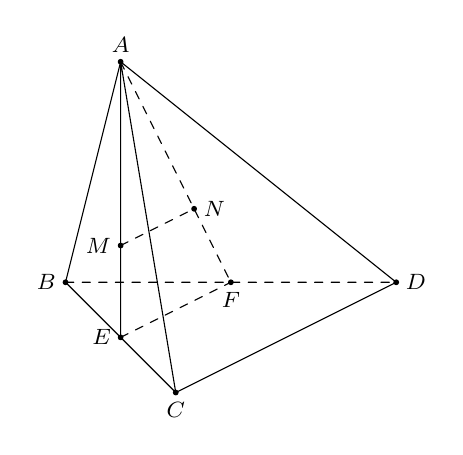
\begin{tikzpicture}[scale=0.7, font=\footnotesize, line join=round, line cap=round, >=stealth]
				\draw[fill=black] (1,4) node[above]{$A$} coordinate (A) circle(1.2pt);
				\draw[fill=black] (0,0) node[left]{$B$} coordinate (B) circle(1.2pt);
				\draw[fill=black] (2,-2) node[below]{$C$} coordinate (C) circle(1.2pt);
				\draw[fill=black] (6,0) node[right]{$D$} coordinate (D) circle(1.2pt);
				\draw[fill=black] (1,-1) node[left]{$E$} coordinate (E) circle(1.2pt);
				\draw[fill=black] (3,0) node[below]{$F$} coordinate (F) circle(1.2pt);
				\draw[fill=black] (1,2/3) node[left]{$M$} coordinate (M) circle(1.2pt);
				\draw[fill=black] (7/3,4/3) node[right]{$N$} coordinate (N) circle(1.2pt);
				\draw (A)--(B)--(C)--(D)--(A) (A)--(E) (A)--(C);
				\draw[dashed] (M)--(N) (E)--(F) (B)--(D) (A)--(F);
		\end{tikzpicture}}
	}
\end{ex}
\begin{ex}[Trích đề thi học kì 1 - THPT Gia Lộc 2 - Hải Dương - Năm học 2024-2025]%[1H4H3-1]%[Dự án dề cương 3 Khối NH24-25-Đợt 3-Võ Thị Thùy Trang]
	Cho đường thẳng $a$ song song với mặt phẳng $(P)$. Khẳng định nào sau đây \textbf{sai}?
	\choice
	{\True $a$ song song với mọi đường thẳng trong $(P)$}
	{$a$ và $(P)$ không có điểm chung}
	{$a$ song song với một đường thẳng nào đó nằm trong $(P)$}
	{Nếu $(Q)$ là mặt phẳng chứa $a$ và cắt $(P)$ theo giao tuyến $b$ thì $b$ song song với $a$}
	\loigiai{Nếu $(Q)$ là mặt phẳng chứa $a$ và cắt $(P)$ theo giao tuyến $b$ thì $b$ song song với $a$. Do đó $a$ song song với mọi đường thẳng trong $(P)$ là khẳng định sai.
	}
\end{ex}
\begin{ex}%[1H4N3-1]%[Dự án dề cương 3 Khối NH24-25-Đợt 3-Võ Thị Thùy Trang]
	Cho hai mặt phẳng $(P)$, $(Q)$ cắt nhau theo giao tuyến là đường thẳng $d$. Đường thẳng $a$ song song với cả hai mặt phẳng $(P)$, $(Q)$. Khẳng định nào sau đây đúng?
	\choice
	{$a$, $d$ trùng nhau}
	{$a$, $d$ chéo nhau}
	{\True $a$ song song $d$}
	{$a$, $d$ cắt nhau}
	\loigiai{
		Sử dụng \textit{hệ quả:} \lq\lq Nếu hai mặt phẳng phân biệt cùng song song với một đường thẳng thì giao tuyến của chúng ( nếu có) cũng song song với đường thẳng đó\rq\rq.
	}
\end{ex}
\begin{ex}%[1H4H3-1]%[Dự án dề cương 3 Khối NH24-25-Đợt 3-Võ Thị Thùy Trang]
	Cho hình hộp $ABCD.A'B'C'D'$. Mệnh đề nào sau đây \textbf{sai}?
	\choice
	{$AB$ song song với $(CDD'C')$}
	{$DD'$ song song với $(ABB'A')$}
	{\True $B'C'$ song song với $(BDD')$}
	{$AD$ song song với $(A'B'C'D')$}
	\loigiai{
		\immini{Ta có $BD\parallel B'D'$ nên $(BDD')\equiv (BB'D'D)$.\\
			$B'=B'C'\cap (BB'D'D)$
			nên $B'C'$ không song song với $(BDD')$.}{
			\begin{tikzpicture}[scale=.4, line join = round, line cap = round]
				\tikzset{label style/.style={font=\footnotesize}}
				\tkzDefPoints{0/0/A,8/0/B,-2/-2/D}
				\coordinate (C) at ($(B)+(D)-(A)$);
				\coordinate (A') at ($(A) - (0,5)$);
				\tkzDefPointsBy[translation = from A to A'](B,C,D){B'}{C'}{D'}
				\tkzDrawPolygon(A,B,B',C',D',D)
				\tkzDrawSegments(C,B C,D C,C' B,D)
				\tkzDrawSegments[dashed](A',A A',B' A',D' B,D')
				\tkzDrawPoints(A,B,D,C,A',B',C',D')
				\tkzLabelPoints[above](A,B)
				\tkzLabelPoints[below](D',C')
				\tkzLabelPoints[left](A',D)
				\tkzLabelPoints[right](B',C)
			\end{tikzpicture}}		}
\end{ex}
\begin{ex}[Trích đề thi học kì 1 - THPT Phan Bội Châu - Lâm Đồng - Năm học 2024-2025]%[1H4H3-2]%[Dự án dề cương 3 Khối NH24-25-Đợt 3-Võ Thị Thùy Trang]
	Cho hình chóp $S.ABCD$. Gọi $M$ và $N$ lần lượt là trung điểm
	của $AB$ và $AD$. Khẳng định nào sau đây đúng?
	\begin{center}
		\begin{tikzpicture}[scale=.7, font=\footnotesize, line join=round, line cap=round, >=stealth]
			\coordinate (A) at (1,1.5);
			\coordinate (B) at (0,0);
			\coordinate (C) at (3,-0.5);
			\coordinate (D) at (5,1.5);
			\coordinate (S) at (0.5,4);
			\coordinate (M) at ($(A)!0.5!(B)$);
			\coordinate (N) at ($(A)!0.5!(D)$);
			\foreach \x/\y in {S/A,A/D,A/B,B/D,M/N,A/C}{
				\draw[dashed] (\x)--(\y);
			}
			\foreach \x/\y in {S/B,S/C,S/D,B/C,C/D}{
				\draw (\x)--(\y);
			}
			\foreach \x in {S,A,B,C,D,M,N}{
				\draw[fill=black] (\x) circle (1pt);
			}
			\foreach \x in {S,B}{
				\node[left] at (\x) {$\x$};
			}
			\foreach \x in {A,N} {
				\node[above right] at (\x) {$\x$};
			}
			\foreach \x in {C,D}{
				\node[right] at (\x) {$\x$};
			}
			\node[above] at (M) {$M$};
		\end{tikzpicture}
	\end{center}
	\choice 
	{$MN\parallel (ABCD)$}
	{$MN\parallel (SCD)$}
	{\True $MN\parallel (SBD)$}
	{$MN\parallel (SAC)$}
	\loigiai{
		Ta có $MN$ là đường trung bình của tam giác $ABD$ nên $MN\parallel BD$.\\ 
		$\heva{&MN\parallel BD\\&MN\not\subset (SBD)\\&BD \subset (SBD)}\Rightarrow MN \parallel (SBD)$.
	}
\end{ex}
\begin{ex}%[1H4N3-2]%[Dự án dề cương 3 Khối NH24-25-Đợt 3-Võ Thị Thùy Trang]
	Cho tứ diện $ABCD$ lấy $I$, $J$ lần lượt là trung điểm của $AB$, $AD$. Đường thẳng $IJ$ song song với mặt phẳng nào dưới đây?
	\choice
	{$(ABD)$}
	{$(ABC)$}
	{$(ACD)$}
	{\True $(CBD)$}
	\loigiai
	{\immini{ Do $IJ$ là đường trung bình của $\triangle ABD$ nên $IJ \parallel BD$.\\
				$\heva{&IJ\parallel BD\\&IJ\not\subset (BCD)\\&BD \subset (BCD)}\Rightarrow IJ \parallel (BCD)$.}
		{\begin{tikzpicture}[scale=0.6, line join = round, line cap = round]
				\tikzset{label style/.style={font=\footnotesize}}
				\tkzDefPoints{0/0/B,8/0/C,2/-3.5/D,3/5/A}
				\coordinate (I) at ($(B)!.5!(A)$); 
				\coordinate (J) at ($(A)!.5!(D)$); 
				\tkzDrawPolygon(A,B,D,C)
				\tkzDrawSegments(A,D I,J)
				\tkzDrawSegments[dashed](B,C)
				\tkzDrawPoints(A,B,C,D,I,J)
				\tkzLabelPoints[above](A)
				\tkzLabelPoints[below](D)
				\tkzLabelPoints[left](B,I)
				%\tkzLabelPoints[below](P)
				\tkzLabelPoints[right](C)
				\tkzLabelPoints[below left](J)
		\end{tikzpicture}}
	}
\end{ex}
\begin{ex}%[1H4H3-2]%[Dự án dề cương 3 Khối NH24-25-Đợt 3-Võ Thị Thùy Trang]
	Cho hình chóp $S.ABCD$, đáy $ABCD$ là hình bình hành tâm $O$. Gọi $M$, $N$ lần lượt là trung điểm của $SB$, $SD$. Trong các mệnh đề sau mệnh đề nào \textbf{sai}?	
	\choice
	{$AM$ không song song với $(SBC)$}
	{$MO$ song song với $(SAD)$}
	{\True $MN$ không song song với $(ABCD)$}
	{$AD$ song song với $(SBC)$}
	\loigiai{
		\immini{
			$MN$ là đường trung bình tam giác $SBD$ nên $MN \parallel BD$.\\
			$\heva{&MN\parallel BD\\&MN\not\subset (ABCD)\\&BD \subset (ABCD)} \Rightarrow MN \parallel (ABCD)$.}{
			\begin{tikzpicture}[scale=0.4, line join = round, line cap = round]
				\tikzset{label style/.style={font=\footnotesize}}
				\tkzDefPoints{0/0/D,7/0/C,3/3/A}
				\coordinate (B) at ($(A)+(C)-(D)$);
				\coordinate (S) at ($(A)+(2,6)$);
				\coordinate (O) at ($(A)!0.5!(C)$);
				\coordinate (M) at ($(S)!0.5!(B)$);
				\coordinate (N) at ($(S)!0.5!(D)$);
				\tkzDrawPolygon(S,B,C,D)
				\tkzDrawSegments(S,C)
				\tkzDrawSegments[dashed](A,S A,B A,D A,C B,D M,N)
				\tkzDrawPoints(D,C,A,B,S,O,M,N)
				\tkzLabelPoints[above](S,O)
				\tkzLabelPoints[left](A,D,N)
				\tkzLabelPoints[right](B,C,M)
			\end{tikzpicture}
	}}
\end{ex}
\begin{ex}%[1H4N3-1]%[Dự án dề cương 3 Khối NH24-25-Đợt 3-Võ Thị Thùy Trang]
	Cho hai đường thẳng $a$ và $b$ chéo nhau. Có bao nhiêu mặt phẳng chứa $a$ và song song với $b$.
	\choice
	{$0$}
	{\True $1$}
	{$2$}
	{Vô số}
	\loigiai{
		Theo định lý \lq\lq Cho hai đường thẳng chéo nhau. Có duy nhất một mặt phẳng chứa đường thẳng này và song song với đường thẳng kia\rq\rq.
	}
\end{ex}
\begin{ex}%[1H4N3-1]%[Dự án dề cương 3 Khối NH24-25-Đợt 3-Võ Thị Thùy Trang]
	Cho hai mặt phẳngg $(P)$, $(Q)$ cắt nhau theo giao tuyến là đường thẳng $d$. Đường thẳng $a$ song song với cả hai mặt phẳng $(P)$, $(Q)$. Khẳng định nào sau đây đúng?
	\choice
	{$a$, $d$ trùng nhau}
	{$a$, $d$ chéo nhau}
	{\True $a$ song song $d$}
	{$a$, $d$ cắt nhau}
	\loigiai{
		Sử dụng \textit{hệ quả:} \lq\lq Nếu hai mặt phẳng phân biệt cùng song song với một đường thẳng thì giao tuyến của chúng (nếu có) cũng song song với đường thẳng đó\rq\rq.
	}
\end{ex}
\begin{ex}%[1H4H3-3]%[Dự án dề cương 3 Khối NH24-25-Đợt 3-Võ Thị Thùy Trang]
	Cho đường thẳng $a\subset (P)$ và đường thẳng $b$ cắt $a$ tại $M$. Mệnh đề nào sau đây là đúng? 
	\choice
	{$b\subset (P)$}
	{$b\cap (P)=\varnothing$}
	{\True Nếu $b\not\subset (P)$ thì $b\cap (P)=M$}
	{$(P)$ là mặt phẳng duy nhất chứa $a$ và $b$}
	\loigiai{
		Cho đường thẳng $a\subset (P)$ và đường thẳng $b$ cắt $a$ tại $M$, suy ra $\heva{&M\in a, a\subset (P)\\ &M\in b.}$\\
		Kết hợp $b\not\subset (P)$ suy ra $b\cap (P)=M$.
	}
\end{ex}
\begin{ex}%[1H4H3-3]%[Dự án dề cương 3 Khối NH24-25-Đợt 3-Võ Thị Thùy Trang]
	Cho hình chóp $S.ABCD$ có đáy $ABCD$ là hình bình hành. Tìm giao tuyến của hai mặt phẳng $(SAD)$ và $(SBC)$.
	\choice
	{$SA$}
	{\True Đường thẳng qua điểm $S$ và song song với $AD$, $BC$}
	{Đường thẳng qua điểm $S$ và song song với $AB$, $CD$}
	{$SO$ với $O$ là giao điểm của $AC$ và $BD$}
	\loigiai{
		\immini{
			Ta có $\heva{&S \in (SAD) \cap (SBC)\\&AD \subset (SAD), BC \subset (SBC)\\&AD \parallel BC}$ nên giao tuyến của hai mặt phẳng $(SAD)$ và $(SBC)$ là đường thẳng $\Delta$ đi qua điểm $S$ và song song với $AD$, $BC$.
		}{\begin{tikzpicture}[declare function={gocx=80; goc=-150; a=5; b=a/2; h=4;}]
			\path (0,0) coordinate (A)--+(gocx:h) coordinate (S)
			(a,0) coordinate (B)
			(goc:b) coordinate (D)
			+(a,0) coordinate (C);
			\path ($(S)+(D)-(A)$) coordinate (E);
			\path ($(E)!1.4!(S)$) coordinate (F);
			\node at (E)[above]{$\Delta$};
			\draw[dashed] (S)--(A) (D)--(A)--(B);
			\draw (S)--(D)--(C)--(S)--(B)--(C)--cycle;
			\draw (E)--(F);
			\foreach \x/\goc in {S/90,A/150,B/0,C/-60,D/-180}
			\draw[fill=white] (\x) node[shift={(\goc:7pt)},font=\scriptsize]{$\x$} circle (1pt);
		\end{tikzpicture}
		}
	}
\end{ex}
\begin{ex}%[1H4H3-1]%[Dự án dề cương 3 Khối NH24-25-Đợt 3-Võ Thị Thùy Trang]
	Trong không gian cho đường thẳng $a$ chứa trong mặt phẳng $(P)$ và đường thẳng $b$ song song với  mặt phẳng $(P)$. Mệnh đề nào sau đây \textbf{sai}?
	\choice
	{$a\parallel b$}
	{$a$, $b$ không có điểm chung}
	{\True $a$, $b$ cắt nhau}
	{$a$, $b$ chéo nhau}	
	\loigiai{
		Từ giả thiết ta suy ra từ tính chất đường thẳng song song với mặt phẳng.	}
\end{ex}
\begin{ex}%[1H4N3-2]%[Dự án dề cương 3 Khối NH24-25-Đợt 3-Võ Thị Thùy Trang]
	\immini{Cho hình chóp $S.ABCD$ có đáy là hình bình hành. Gọi $M$, $N$ là trung điểm $AB$, $CD$ (như hình vẽ). Tìm mệnh đề đúng.
		\choice
		{\True $MN \parallel (SBC)$}
		{$MN \parallel (SAB)$}
		{$MN \parallel (SCD)$}
		{$MN \parallel (ABCD)$}
	}{
		\begin{tikzpicture}[scale=0.8, line join=round, line cap=round]
			\path
			(0,0) coordinate (A)
			(-1.3,-1.6) coordinate (B)
			(2.5,-1.6) coordinate (C)
			;
			\coordinate (D) at ($(A)+(C)-(B)$);
			\coordinate (S) at ($(A)+(-0.3,3)$);
			\coordinate (M) at ($(A)!0.5!(B)$);
			\coordinate (N) at ($(C)!0.5!(D)$);
			\draw[dashed] (S)--(A)--(B) (A)--(D) (M)--(N);
			\draw (S)--(B)--(C)--(D)--(S)--(C);
				\foreach \t/\goc in {A/45,B/-90,C/-90,D/0,N/0,S/90,M/90}{
				\fill (\t) circle (1pt) node[font=\scriptsize,shift={(\goc:9pt)}] {$\t$};
			}
		\end{tikzpicture}
	}
	\loigiai{
		Ta có $\heva{&MN\parallel BC\\&BC\subset (SBC)\\&MN \not\subset (SBC)} \Rightarrow MN \parallel (SBC)$.}
\end{ex}
\Closesolutionfile{ans}
\ind{PHẦN II.} \inden{Câu trắc nghiệm đúng sai. Trong mỗi ý a), b), c), d) ở mỗi câu, học sinh chọn đúng hoặc sai.}\\
\setcounter{ex}{0}
\Opensolutionfile{ans}[ans/1H4-Bai3-DS]
\begin{ex}%[1H4H3-2]%[Dự án dề cương 3 Khối NH24-25-Đợt 3-Võ Thị Thùy Trang]
	Cho hình chóp $S.ABCD$ đáy $ABCD$ là hình bình hành. Gọi $I$, $J$ lần lượt là trọng tâm của tam giác $SAB$ và $SCD$, $E$, $F$ lần lượt là trung điểm của $AB$ và $CD$. Khi đó
	\choiceTF
	{\True $\dfrac{SJ}{SF}=\dfrac{2}{3}$}
	{\True $IJ\parallel (ABCD)$}
	{\True $BC$ song song với mặt phẳng $(SAD)$, $(SEF)$}
	{$BC$ cắt mặt phẳng $(AIJ)$}														
	\loigiai{
		\begin{center}
			\begin{tikzpicture}[>=stealth,line join=round,line cap=round,scale=1.5]
				\draw[dashed,black,scale=2.5] (0,0)coordinate(A)--(-130:0.5)coordinate(B) (1,0)coordinate(D)--(A)--($(A)+(80:1)$)coordinate(S);
				\coordinate (E) at ($(A)!0.5!(B)$);
				\coordinate (F) at ($(C)!0.5!(D)$);
				\coordinate (I) at ($(S)!2/3!(E)$);
				\coordinate (J) at ($(S)!2/3!(F)$);
				\draw[dashed](S)--(E)--(F) (I)--(J);
				\draw[black,scale=2.5] (B)--($(D)-(A)+(B)$)coordinate(C)--(D)--(S)--(B) (S)--(C) (S)--(F);
				\foreach \diem/\vitrin in {S/above,A/above right,B/below left,C/below right,D/right,F/right,E/below right,I/above right,J/right} \fill (\diem)circle(.75pt)node[\vitrin]{$\diem$};
			\end{tikzpicture}
		\end{center}	
		\begin{itemchoice}
			\itemch \textbf{Đúng}.\\
			 Do $I$, $J$ lần lượt là trọng tâm của tam giác $SAB$ và $SCD$ nên $\dfrac{SI}{SE}=\dfrac{SJ}{SF}=\dfrac{2}{3}$.
			\itemch \textbf{Đúng}.\\
			 Vì $\dfrac{SI}{SE}=\dfrac{SJ}{SF}=\dfrac{2}{3}$ nên $IJ\parallel EF$. Mà $EF\subset (ABCD)\Rightarrow IJ\parallel (ABCD)$.
			\itemch \textbf{Đúng}.\\
			 Vì $BC\parallel AD$, $AD\subset (SAD)\Rightarrow BC\parallel (SAD)$.
			Vì $EF$ là đường trung bình của hình bình hành $ABCD$ nên
			$BC\parallel EF$, $EF\subset (SEF)\Rightarrow BC\parallel (SEF)$.
			\itemch \textbf{Sai}.\\
			 Ta có $IJ\parallel EF$, $EF\parallel BC\Rightarrow BC\parallel IJ$ mà $IJ\subset (AIJ)\Rightarrow BC\parallel (AIJ)$.
		\end{itemchoice}		
	}
\end{ex}
\begin{ex}%[1H4H3-2]%[Dự án dề cương 3 Khối NH24-25-Đợt 3-Võ Thị Thùy Trang]
	Cho hình chóp tứ giác đều $S.ABCD$ có cạnh đáy bằng $2$, $M$ là một điểm thuộc cạnh $SA$ sao cho $\dfrac{SM}{SA}=\dfrac{2}{3}$. Một mặt phẳng $(\alpha)$ đi qua $M$ song song với $AB$ và $AD$, cắt các mặt của hình chóp theo hình là một tứ giác.										
	\choiceTF
	{\True Giao tuyến của mặt phẳng $(\alpha)$ với mặt phẳng $(SAB)$ là đường thẳng đi qua $M$ và song song với $AB$}
	{Giao tuyến của mặt phẳng $(\alpha)$ với mặt phẳng $(SAD)$ là đường thẳng đi qua $M$ và song song với $SD$}
	{$\dfrac{SM}{SA}=\dfrac{1}{3}$}
	{\True Mặt phẳng $(\alpha)$ đi qua $M$ song song với $AB$ và $AD$, cắt các mặt của hình chóp theo hình là một tứ giác có diện tích bằng $\dfrac{16}{9}$}
	\loigiai{\begin{center}
			\begin{tikzpicture}[>=stealth,line join=round,line cap=round,scale=1.5]
				\draw[dashed,black,scale=2.5] (0,0)coordinate(A)--(-130:0.5)coordinate(B) (1,0)coordinate(D)--(A)--($(A)+(80:1)$)coordinate(S);
				\coordinate (M) at ($(S)!2/3!(A)$);
				\coordinate (N) at ($(S)!2/3!(B)$);
				\coordinate (P) at ($(S)!2/3!(C)$);
				\coordinate (Q) at ($(S)!2/3!(D)$);
				\draw[dashed](Q)--(M)--(N);
				\draw[black,scale=2.5] (B)--($(D)-(A)+(B)$)coordinate(C)--(D)--(S)--(B) (S)--(C)
				(N)--(P)--(Q);
				\foreach \diem/\vitrin in {S/above,A/left,B/below left,C/below right,D/right,N/left,M/above right,P/below left,Q/right} \fill (\diem)circle(.75pt)node[\vitrin]{$\diem$};
			\end{tikzpicture}
		\end{center}
		\begin{itemchoice}
			\itemch \textbf{Đúng}.\\
			 Vì $\heva{&M\in (SAB)\cap (\alpha)\\&(\alpha)\parallel AB,\,AB\subset (SAB)}$\\ $\Rightarrow (SAB)\cap (\alpha)=MN$ với $MN\parallel AB$, $N\in SB$.
			\itemch \textbf{Sai}.\\
			 $\heva{&M\in (SAD)\cap (\alpha)\\&(\alpha)\parallel AD, \,AD\subset (SAD)}\Rightarrow (SAD)\cap (\alpha)=MQ$ với $MQ\parallel AD$, $Q\in SD$.
			\itemch \textbf{Sai}.\\
			 Vì $BC\parallel AD\parallel MQ$ và $BC\not \subset (\alpha)$, $MQ\subset (\alpha)$ nên $BC\parallel (\alpha)$.\\
			Khi đó, ta có $\heva{&N\in (SBC)\cap (\alpha)\\&(\alpha)\parallel BC,\,BC\subset (SBC)}$\\ 
			$\Rightarrow (SBC)\cap (\alpha)=NP$ (với $NP\parallel BC$, $P\in SC$).\\
			Nối các đỉnh $M$, $N$, $P$, $Q$ ta được một tứ giác.\\
			Ta có $MN\parallel AB$, $MQ\parallel AD$, $NP\parallel BC$, $PQ\parallel CD$ nên theo định lí Thalès, ta có
			\[\dfrac{SM}{SA}=\dfrac{SN}{SB}=\dfrac{SP}{SC}=\dfrac{SQ}{SD}=\dfrac{MN}{AB}=\dfrac{NP}{BC}=\dfrac{PQ}{CD}=\dfrac{MQ}{AD}=\dfrac{2}{3}.\]
			\itemch \textbf{Đúng}.\\
			 $MN=NP=PQ=MQ=\dfrac{2}{3} \cdot 2=\dfrac{4}{3}$ (đáy hình của chóp là hình vuông cạnh $2$).\\
			Dễ thấy $MNPQ$ là một hình vuông có cạnh bằng $\dfrac{4}{3}$ nên có diện tích bằng $\dfrac{16}{9}$ (đơn vị diện tích).
	\end{itemchoice}			}
\end{ex}
\begin{ex}%[1H4H3-3]%[Dự án dề cương 3 Khối NH24-25-Đợt 3-Võ Thị Thùy Trang]
	Cho hình chóp $S.ABCD$ có đáy $ABCD$ là hình bình hành. Lấy điểm $M$ trên cạnh $AD$ sao cho $AD=3AM$. Gọi $G$, $N$ theo thứ tự là trọng tâm các tam giác $SAB$, $ABC$. Khi đó														
	\choiceTF
	{Giao tuyến của hai mặt phẳng $(SAB)$ và $(SCD)$ là đường thẳng đi qua $S$ và song song với $AC$, $BD$}
	{$\dfrac{DN}{DB}=\dfrac{1}{3}$}
	{\True $MN$ song song với mặt phẳng $(SCD)$}
	{$NG$ cắt với mặt phẳng $(SAC)$}
	\loigiai{\begin{center}
			\begin{tikzpicture}[>=stealth,line join=round,line cap=round,scale=1.5]
				\draw[dashed,black,scale=2.5] (0,0)coordinate(A)--(-130:0.5)coordinate(B) (1,0)coordinate(D)--(A)--($(A)+(80:1)$)coordinate(S);
				\coordinate(O) at ($(A)!0.5!(C)$);
				\coordinate (M) at ($(A)!1/4!(D)$);
				\coordinate (x) at ($(S)+(B)-(A)$);
				\coordinate (P) at ($(A)!1/2!(B)$);
				\coordinate (G) at ($(S)!2/3!(P)$);
				\coordinate (y) at ($(S)!-2/3!(x)$);
				\path (intersection of P--C and B--O) coordinate (N);
				\draw[black,scale=2.5] (B)--($(D)-(A)+(B)$)coordinate(C)--(D)--(S)--(B) (S)--(C) (y)--(S)--(x);
				\draw[dashed](A)--(C) (B)--(D) (S)--(P)--(C) (M)--(N)--(G);
				\foreach \diem/\vitrin in {S/above,A/left,B/below left,C/below right,D/right,O/below,M/above right,P/below left,N/below,G/right,x/left} \fill (\diem)circle(.75pt)node[\vitrin]{$\diem$};
			\end{tikzpicture}
		\end{center}
		\begin{itemchoice}
			\itemch \textbf{Sai}.\\
			 Ta có $\heva{&S\in (SAB)\cap (SCD)\\&AB\parallel CD\\&AB\subset (SAB),CD\subset (SCD)}\Rightarrow (SAB)\cap (SCD)=Sx$.\\ (với $Sx$ qua $S$ và $Sx\parallel AB\parallel CD$).
			\itemch \textbf{Sai}.\\
			 Gọi $O$ là tâm hình bình hành $ABCD$.
			Vì $N$ là trọng tâm của $\triangle ABC$ nên $BN=\dfrac{2}{3}BO=\dfrac{2}{3} \cdot \dfrac{1}{2} BD=\dfrac{1}{3} BD\Rightarrow \dfrac{DN}{DB}=\dfrac{2}{3}$.
			\itemch \textbf{Đúng}.\\
			 Ta có $AD=3AM\Rightarrow \dfrac{DM}{DA}=\dfrac{2}{3}$.\\
			Xét tam giác $ADB$, ta có $\dfrac{DM}{DA}=\dfrac{DN}{DB}=\dfrac{2}{3}$ nên\\ $MN\parallel AB\Rightarrow MN\parallel CD$,
			mà $CD\subset (SCD)\Rightarrow MN\parallel (SCD)$.
			\itemch \textbf{Sai}.\\
			 Gọi $P$ là trung điểm $AB$. Tam giác $SPC$ có
			$\dfrac{PG}{PS}=\dfrac{PN}{PC}=\dfrac{1}{3}$ (tính chất trọng tâm)
			\[\Rightarrow NG\parallel SC,\,SC\subset (SAC)\Rightarrow NG\parallel (SAC).
			\]
		\end{itemchoice}		
	}
\end{ex}																
\begin{ex}%[1H4H3-3]%[Dự án dề cương 3 Khối NH24-25-Đợt 3-Võ Thị Thùy Trang]
	Cho hình chóp $S.ABC$. Gọi $I$, $J$ lần lượt là trung điểm của $AB$ và $BC$. Gọi $H$, $K$ lần lượt là trọng tâm của $\triangle SAB$ và $\triangle SBC$. Khi đó
	\choiceTF
	{\True $AC\parallel (SIJ)$}
	{$HK$ cắt $IJ$}
	{\True $HK\parallel (SAC)$}
	{\True Giao tuyến của $(BHK)$ và $(ABC)$ là đường thẳng đi qua $B$ và song song với $AC$}																		
	\loigiai{
		\begin{center}
			\begin{tikzpicture}[>=stealth,line join=round,line cap=round,scale=1.5]
				\draw[black,scale=2.5] (0,0)coordinate(A)--(-35:0.8)coordinate(B)--(1,0)coordinate(C)--($(A)+(70:1)$)coordinate(S)--(B) (S)--(A);
				\coordinate (I) at ($(A)!0.5!(B)$);
				\coordinate (J) at ($(C)!0.5!(B)$);
				\coordinate (M) at ($(S)!0.5!(B)$);
				\path (intersection of A--M and S--I) coordinate (H);
				\path (intersection of M--C and S--J) coordinate (K);
				\draw[dashed,black,scale=2.5]  (A)--(C) (I)--(J) (H)--(K);
				\draw (S)--(I) (S)--(J) (A)--(M)--(C);
				\foreach \diem/\vitrin in {S/above,A/left,B/below left,C/right,I/below,J/right,H/left,K/right}	\fill (\diem)circle(.75pt)node[\vitrin]{$\diem$};
			\end{tikzpicture}
		\end{center}
		\begin{itemchoice}
			\itemch \textbf{Đúng}.\\
			 Vì $IJ$ là đường trung bình $\triangle ABC$ nên $IJ\parallel AC$.\\
			Ta có $\heva{&AC\parallel IJ\\&IJ\subset (SIJ)\\&AC\not \subset (SIJ)} \Rightarrow AC\parallel (SIJ)$.
			\itemch \textbf{Sai}.\\
			 Ta có $\dfrac{SH}{HI}=\dfrac{SK}{KJ}=2$ ($H$, $K$ lần lượt là trọng tâm $\triangle SAB$ và $\triangle SAC)$.
			$\Rightarrow HK\parallel IJ$.
			\itemch \textbf{Đúng}.\\
			 Ta có $\heva{&HK\parallel AC \,(HK\parallel IJ,\,AC\parallel IJ)\\&AC\subset (SAC)\\&HK\not \subset (SAC)} \Rightarrow HK\parallel (SAC)$.
			\itemch \textbf{Đúng}.\\
			 Ta có $\heva{&HK\parallel AC\\&HK\subset (BHK)\\&AC\subset (ABC)\\&B\in (BHK)\cap (ABC).}$\\
			Vậy giao tuyến của $(BHK)$ và $(ABC)$ là đường thẳng $Bx$ đi qua $B$ và song song với $AC$ và $HK$.
	\end{itemchoice}			}
\end{ex}							
\begin{ex}[Trích đề thi học kì 1 - THPT Tân Châu - An Giang - Năm học 2024-2025]%[1H4V3-3]%[Dự án dề cương 3 Khối NH24-25-Đợt 3-Võ Thị Thùy Trang]
	Cho hình chóp $S.ABCD$ có đáy $ABCD$ là hình bình hành. Gọi $M$ là điểm thuộc cạnh $SA$ sao cho $SM=\dfrac{1}{3}SA$ và $N$ là điểm thuộc cạnh $SD$ sao cho $SN=\dfrac{2}{3}SD$. 
	\choiceTF
	{Hai đường thẳng $SA$ và $BC$ cắt nhau}
	{\True $BC$ song song với mặt phẳng $(SAD)$}
	{Giao tuyến của hai mặt phẳng $(SAB)$ và $(SCD)$ là đường thẳng đi qua $S$ và song song với $AD$}
	{\True Giao điểm của đường thẳng $MN$ và mặt phẳng $(ABCD)$ là điểm $P$ với $P=MN \cap AD$}
	\loigiai{
		\begin{center}
			\begin{tikzpicture}[>=stealth,line join=round,line cap=round,font=\footnotesize,scale=1]
				\tikzset{
					pics/hinhChopTuGiac/.style n args={5}{
						code={
							\tikzset{
								declare function={a=4;b=2;h=3;goc=-120;}
							}	
							\path 
							(0,0)coordinate(#1)+(0:a)coordinate(#2)+(goc:b)coordinate(#4)+(110:h)coordinate(#5)
							($(#2)+(#4)-(#1)$)coordinate(#3)
							;
						}
				}}
				\path 
				(0,0)pic{hinhChopTuGiac={A}{B}{C}{D}{S}}
				($(S)!1/3!(A)$)coordinate(M)
				($(S)!2/3!(D)$)coordinate(N)
				(intersection of M--N and A--D) coordinate(P)
				;	
				\foreach \pointo/\pointt in{S/B,S/C,S/D,D/C,C/B,N/P,D/P}{
					\draw[fill=black](\pointo)--(\pointt);
				}
				\foreach \pointo/\pointt in{S/A,A/B,A/D,M/N}{
					\draw[fill=black,dashed](\pointo)--(\pointt);
				}
				\foreach \point/\goc in{A/180,S/90,D/-80,B/10,C/-45,M/-5,N/150,P/180}{
					\draw[fill=black](\point)circle(.8pt)+(\goc:2mm)node[scale=.8]{$\point$};
				}
			\end{tikzpicture}
		\end{center}
		\begin{itemchoice}
			\itemch \textbf{Sai}.\\
			Đường thẳng $SA$ nằm trong mặt phẳng $(SAD)$. Đường thẳng $BC$ song song với $AD$(do $ABCD$ là hình bình hành), mà $AD \subset(SAD)$, $BC \not\subset(SAD)$, nên $BC \parallel(SAD)$.\\
			Do đó, $BC$ và $SA$ là hai đường thẳng chéo nhau(không đồng phẳng), chúng không thể cắt nhau.			
			\itemch \textbf{Đúng}.\\
			Ta có $\heva{
				& BC \parallel AD \\
				& AD \subset(SAD) \\
				& BC \not\subset(SAD)
			} \Rightarrow BC \parallel(SAD)$.
			\itemch \textbf{Sai}.\\
			Ta có $\heva{&S \in(SAB) \cap(SCD) \\ &AB \subset(SAB), CD \subset(SCD) \\ &AB \parallel CD}$\\
			Do đó, giao tuyến của hai mặt phẳng $(SAB)$ và $(SCD)$ là đường thẳng $d$ đi qua $S$ và song song với $AB$(và $CD$).
			\itemch \textbf{Đúng}.\\
			Trong $\triangle SAD$, ta có $\dfrac{SM}{SA}=\dfrac{1}{3}$ và $\dfrac{SN}{SD}=\dfrac{2}{3}$.\\
			Vì $\dfrac{SM}{SA} \ne \dfrac{SN}{SD}$, theo định lý Thales đảo, đường thẳng $MN$ không song song với $AD$. \\
			Khi đó $MN\cap AD=P$, nên $M\in MN$ và $M\in AD\subset(ABCD)$.\\
			Do đó $P$ chính là giao điểm của $MN$ và mặt phẳng $(ABCD)$, và $P=MN \cap AD$.
		\end{itemchoice}
	}
\end{ex}
\Closesolutionfile{ans}
\ind{PHẦN III.} \inden{Câu trắc nghiệm trả lời ngắn}\\
\setcounter{ex}{0}
\Opensolutionfile{ans}[ans/1H4-Bai3-TLN]
\begin{ex}%[1H4H3-2]%[Dự án dề cương 3 Khối NH24-25-Đợt 3-Võ Thị Thùy Trang]	
	Cho hình chóp $S.ABCD$ có đáy $ABCD$ là hình bình hành tâm $O$. Mặt phẳng $(\alpha)$ đi qua trung điểm $I$ của $OA$ song song với $BD$ và song song với $SC$, $(\alpha)$ cắt $SA$ tại $K$. Xác định $\dfrac{AK}{SK}$.\par
	\shortans{3}
	\loigiai{
		\immini{
			$O$ trung điểm $AC$, $I$ là trung điểm $AO$ nên $\dfrac{AI}{AC}=\dfrac{1}{4}$.\\
			$(\alpha)$ là mặt phẳng song song với $BD$ nên $MN \parallel BD$ và $(\alpha)$ song song với $SC$ nên $KI \parallel SC$.\\
		    $\dfrac{AK}{AS}=\dfrac{AI}{AC}=\dfrac{1}{4}$.\\
			Nên $AK=3SK$.}
		{\begin{tikzpicture}[declare function={gocx=80; goc=-150; a=5; b=a/2; h=4.5;}]
				\path (0,0) coordinate (A)--+(gocx:h) coordinate (S)
				(a,0) coordinate (B)
				(goc:b) coordinate (D)
				+(a,0) coordinate (C);
				\path ($(A)!0.5!(C)$) coordinate (O);
				\path ($(A)!0.5!(O)$) coordinate (I);
				\path ($(A)!0.5!(B)$) coordinate (M);
				\path ($(A)!0.5!(D)$) coordinate (N);
				\path ($(A)!0.25!(S)$) coordinate (K);
				\draw[dashed] (S)--(A) (D)--(A)--(B) (A)--(C) (B)--(D) (M)--(N)--(K)  (I)--(K)--(M);
				\draw (S)--(D)--(C)--(S)--(B)--(C)--cycle;
				\foreach \x/\goc in {S/90,A/150,B/0,C/-60,D/-180,O/-90,I/-90,M/90,N/90,K/180}
				\draw[fill=white] (\x) node[shift={(\goc:7pt)},font=\scriptsize]{$\x$} circle (1pt);
		\end{tikzpicture}}
	}
\end{ex}
\begin{ex}%[1H4H3-3]%[Dự án dề cương 3 Khối NH24-25-Đợt 3-Võ Thị Thùy Trang]
	Cho hình chóp $S.ABCD$ có đáy $ABCD$ là hình bình hành tâm $O$, $M$ là trung điểm đoạn $SB$, $G$ là trọng tâm tam giác $SAD$. Gọi $J$ là giao điểm của $AD$ với $(OMG)$. Tính $\dfrac{AD}{JD}$.\par 
		\shortans{3}
	\loigiai{
		\immini{Ta có $MO$ là đường trung bình của tam giác $SBD$ suy ra $MO\parallel SD$.\\
			Ta có $\left\{
			\begin{aligned}&MO\parallel SD\\ &G\in (OMG)\cap (SAD) \end{aligned}\right.\\
			\Rightarrow (OMG)\cap (SAD)=Gx\parallel SD\parallel MO\\ \Rightarrow Gx\cap AD=J$.\\
			Ta có $J\in Gx\subset (OMG)\Rightarrow J=AD\cap (OMG)$.\\
			Gọi $E$ là trung điểm $SD$ với $G$ là trọng tâm ta có $\dfrac{AG}{AE}=\dfrac{2}{3}$.\\
				Do $GJ\parallel MO\parallel SD$ nên ta có $\dfrac{AE}{GE}=\dfrac{AD}{JD}=3$.}
			{\begin{tikzpicture}[scale=.7,declare function={gocx=80; goc=-150; a=5; b=a/2; h=4;}]
					\path (0,0) coordinate (A)--+(gocx:h) coordinate (S)
					(a,0) coordinate (B)
					(goc:b) coordinate (D)
					+(a,0) coordinate (C);
					\path ($(A)!0.5!(C)$) coordinate (O);
					\path ($(S)!0.5!(B)$) coordinate (M);
					\path ($(S)!0.5!(D)$) coordinate (E);
					\path (barycentric cs:A=1,D=1,S=1) coordinate (G);
					\path ($(A)!2/3!(D)$) coordinate (J);
					\draw[dashed] (S)--(A) (D)--(A)--(B) (A)--(C) (B)--(D) (O)--(M)--(G)--(O) (A)--(E) (G)--(J);
					\draw (S)--(D)--(C)--(S)--(B)--(C)--cycle;
					\foreach \x/\goc in {S/90,A/150,B/0,C/-60,D/-180,O/-90,M/90,G/180,E/180,J/180}
					\fill (\x) node[shift={(\goc:7pt)},font=\scriptsize]{$\x$} circle (1pt);
			\end{tikzpicture}}
	}
\end{ex}
\begin{ex}[Trích đề thi học kì 1 - THPT DakLak - Năm học 2024-2025]%[1H4V3-2]%[Dự án dề cương 3 Khối NH24-25-Đợt 3-Võ Thị Thùy Trang]
	Trong không gian, cho hình chóp $S.ABCD$ có đáy $ABCD$ là hình thang với $AB$ là đáy lớn. Biết $AB=7a$, $CD=3a$. Gọi $I$ là điểm thuộc cạnh $SB$ thỏa mãn $\dfrac{IS}{IB}=\dfrac{x}{y}$ (với $x$, $y$ là các số nguyên dương và $\dfrac{x}{y}$ là phân số tối giản). Biết rằng $CI$ song song với mặt phẳng $(SAD)$. Giá trị của $x+y$ bằng bao nhiêu?\par
	\shortans{7}
	\loigiai{\begin{center}
			\begin{tikzpicture}[line join=round, line cap=round,>=stealth,font=\footnotesize,scale=0.9]
				\def\a{6}
				\def\b{2}
				\def\h{3.4}
				\path 	(0:0) coordinate (A)
				++(0:\a) coordinate (B)
				(A)++(-70:\b) coordinate (D)
				++(0:3*\a/7) coordinate (C)
				($(A)+(70:\h)$) coordinate (S)
				($(S)!3/7!(B)$) coordinate (I)
				($(S)!3/7!(A)$) coordinate (J);
				\draw[dashed,thick] (A)--(B) (I)--(J);
				\draw[thick] (S)--(A)--(D)--(C)--(B)--(S)--(D) (S)--(C)--(I) (D)--(J);
				\foreach \x/\g in {A/180,D/180,C/0,B/0,S/180,I/0,J/180}
				\fill[black] (\x) circle (1pt) ($(\g:4mm)+(\x)$) node {$\x$};	
			\end{tikzpicture}
		\end{center}
		Kẻ $IJ \parallel AB$ với $J \in SA$.\\
		Mà $AB \parallel CD$ nên $IJ \parallel CD$. \quad (1)\\
		Ta có $\heva{&CI \parallel (SAD)\\&DJ \subset (SAD)} \Rightarrow CI \parallel DJ$. \quad (2)\\
		Từ (1) và (2) suy ra $JICD$ là hình bình hành.\\
		Khi đó $IJ=CD=3a$.\\
		Ta có $\dfrac{SI}{SB}=\dfrac{IJ}{AB}=\dfrac{3a}{7a}=\dfrac{3}{7} \Rightarrow \dfrac{SI}{IB}=\dfrac{3}{4}$.\\
		Vậy $x=3$, $y=4$ nên $x+y=7$.}
\end{ex}
\begin{ex}[Trích đề thi học kì 1 - THPT DTNT - Phú Yên - Năm học 2024-2025]%[1H4V3-3]%[Dự án dề cương 3 Khối NH24-25-Đợt 3-Võ Thị Thùy Trang]
	Cho hình chóp $S. ABCD$ có đáy $ABCD$ là hình bình hành. Gọi $M$ là trung điểm cạnh $BC$, $(\alpha)$ là mặt phẳng qua $A$, $M$ và song song với $SD$. Mặt phẳng $(\alpha)$ cắt $SB$ tại $N$, tính tỉ số $\dfrac{S N}{SB}$ (làm tròn đến hàng phần trăm).\par
	\shortans{0{,}67}
	\loigiai{
		\begin{center}
			\begin{tikzpicture}
				\def\a{4}
				\path 	(0:0) coordinate (A)
				++(0:\a) coordinate (B)
				++(-140:.6*\a) coordinate (C)
				($(A)+(C)-(B)$) coordinate (D)
				($(A)+(80:\a)$) coordinate (S)
				(intersection of A--C and B--D) coordinate (O)
				($(B)!.5!(C)$) coordinate (M)
				(intersection of A--M and B--D) coordinate (G)
				($(B)!1/3!(S)$) coordinate (N);
				\draw[dashed] 	(B)--(A)--(D)	(A)--(S) (A)--(M) (D)--(B) (A)--(C) (G)--(N)--(A);
				\draw	(B)-- (C)--(D)
				(B)--(S)	(C)--(S)	(D)--(S) (M)--(N);
				\foreach \x/\g in {A/135,B/-45,C/-45,D/-135,S/90,M/-45,N/60,G/-75,O/-90}
				\fill[black] 	(\x) circle (1pt)
				($(\g:3mm)+(\x)$) node {$\x$};	
			\end{tikzpicture}
		\end{center}
		Gọi $O$ là tâm hình bình hành $ABCD$, $G$ là giao điểm của $OB$ và $AM$ thì $G$ là trọng tâm $\triangle ABC$.\\
		Ta có $\heva{&(\alpha)\parallel SD\\&SD\subset(SBD)\\&(SBD)\cap(\alpha)=Gx\parallel SD.}$\\
		Trong mặt phẳng $(SBD)$, gọi $N$ là giao điểm của $Gx$ và $SB$ thì $GN\parallel SD$.\\
		Khi đó $\dfrac{SN}{SB}=\dfrac{DG}{DB}=\dfrac{2}{3}\approx0{,}67$ (do $G$ là trọng tâm $\triangle ABC$).
	}
\end{ex}
\begin{ex}[Trích đề thi học kì 1 - Sở Giáo dục và Đào tạo Bắc Giang - Năm học 2024-2025]%[1H4V4-3]%[Dự án dề cương 3 Khối NH24-25-Đợt 3-Võ Thị Thùy Trang]
	Cho hình chóp $S.ABCD$ có đáy $ABCD$ là hình thang với $AB\parallel CD$ và $AB > CD$. Biết $AB = 5a$, $CD = 3a$. Gọi $E$ là điểm thuộc cạnh $SB$ sao cho đường thẳng $CE$ song song với mặt phẳng $(SAD)$. Biết tỉ số $\dfrac{ES}{EB} = \dfrac{m}{n}$ với $\dfrac{m}{n}$ là phân số tối giản $(m, n \in N^*)$. Tính giá trị của biểu thức $2m+3n$.\par
	\par\shortans{$12$}
	\loigiai{
		\immini
		{Gọi $K\in AB$ sao cho $CK\parallel AD$.\\
			Ta có $CK\parallel AD$ và $CD\parallel AK$ nên tứ giác $ADCK$ là hình bình hành.\\
			Suy ra $AK=CD=3a$. Suy ra $KB=2a$.\\
			Đồng thời, do $AD\subset (SAD)$ nên $CK\parallel (SAD)$. Suy ra $CK\parallel SA$.\\
			Trong $\triangle SAB$, kẻ $KE\parallel SA$, ta có
			$$\heva{&KE\parallel SA \\& CK\parallel SA \\& KE\cap CK=K\in(KEC).}$$
		}
		{\tdplotsetmaincoords{75}{100} % Đặt góc nhìn
			\begin{tikzpicture}[font=\footnotesize, line join=round, line cap=round, >=stealth, tdplot_main_coords, scale=1]
				\def\a{0.7}
				\path
				(0,0,0) coordinate (A)+(0,3*\a,0) coordinate (K)+(0,5*\a,0) coordinate (B)
				(3,2,0) coordinate (D)++(0,3*\a,0) coordinate (C)
				(2,1,3) coordinate (S) ($(S)!3/5!(B)$) coordinate (E);
				\draw (S)--(A)--(D)--(C)--(B)--cycle (D)--(S)--(C)--(E);
				\draw[dashed] (A)--(B) (C)--(K)--(E);
				\foreach \x/\g in {S/above, A/left, B/right, C/below right, D/below left, K/above left, E/right}{
					\fill (\x) circle (1pt)node[\g]{$\x$};
				}
		\end{tikzpicture}}\
		Suy ra $SA\parallel (KEC)$. Do đó $SA\parallel CE$.\\
		Nên $CE\parallel (SAD)$.\\
		Suy ra điểm $E\in SB$ cần tìm thỏa $KE\parallel SA$.\\
		Do đó $\dfrac{ES}{EB}=\dfrac{KA}{KB}=\dfrac{3a}{2a}=\dfrac{3}{2}$.\\
		Suy ra $m=3$, $n=2$.\\ Vậy $2m+3n=2\cdot3+3\cdot2=12$.
	}
\end{ex}
\Closesolutionfile{ans}
\ind{PHẦN IV.} \inden{Tự luận.}
\setcounter{ex}{0}
\begin{ex}%[1H4H3-1]%[Dự án dề cương 3 Khối NH24-25-Đợt 3-Võ Thị Thùy Trang]
	\immini{Mô tả vị trí tương đối của các đường thẳng $a$, $b$, $c$, $d$, $e$ với mặt phẳng $(P)$ là mặt trước của tòa nhà (hình bên).}{\begin{tikzpicture}[line join=round, line cap=round,scale=1,transform shape]
			\definecolor{amber(sae/ece)}{rgb}{1.0, 0.49, 0.0}
			\definecolor{ceruleanblue}{rgb}{0.16, 0.32, 0.75}
			\definecolor{darkgray}{rgb}{0.66, 0.66, 0.66}
			\definecolor{cottoncandy}{rgb}{1.0, 0.74, 0.85}
			\begin{scope}[scale=.7]
				\clip (-5.5,-3.5) rectangle (7.3,2.55);
				
				\tikzset{building/.pic={
						\def\b{
							(-6,6)--(-.7,6)--(-.7,1.2)--(3,1.2)--(3,-5)--(-6,-5)--cycle %tường lớn xanh
							;}
						\fill[color=ceruleanblue] \b;
						\draw[color=yellow,line width=1] %(-6,2)--(-.7,2)
						(-6,1)--(3,1) (0,0)--(3,0) (0,-1)--(3,-1) (0,-2)--(3,-2);
						\draw \b;
						\draw[fill=yellow] (-.7,1.2)--(3,1.2)--(3,1.5)--(-.7,1.5)--cycle; %ô vàng
						
						\def\c{
							(-6,0)--(0,0)--(0,-3)--(3,-3)--(3,-5)--(-6,-5)--cycle %tường lớn
							;}
						\fill[color=amber(sae/ece)!80] \c; %tô cam
						\draw[color=amber(sae/ece),line width=1] (-6,-2)--(0,-2) (-6,-3)--(0,-3); %sọc cam
						
						%%%%CỬA SỔ 1
						\fill[color=darkgray] (-2,-1.5)--(-2,-3.2)--(-.5,-3.2)--(-.5,-1.5)--cycle; %viền cửa sổ
						\draw[color=yellow,line width=1] (-1.25,-1.5)--(-1.25,-3.2);
						\draw[color=amber(sae/ece),line width=1](-6,-1)--(0,-1)  (-6,-4)--(3,-4);
						\draw[fill=yellow] (-2,-3)--(-2,-3.2)--(-.5,-3.2)--(-.5,-3)--cycle; %ô vàng dưới cửa sổ 
						\draw (-2,-1.5)--(-2,-3.2)--(-.5,-3.2)--(-.5,-1.5)--cycle; %viền cửa sổ
						
						%%%%CỬA SỔ 2
						\fill[color=darkgray] (-5,-1.5)--(-5,-3.2)--(-3.5,-3.2)--(-3.5,-1.5)--cycle; %viền cửa sổ
						\draw[color=yellow,line width=1] (-4.25,-1.5)--(-4.25,-3.2);
						%\draw[color=amber(sae/ece),line width=1](-6,-1)--(0,-1)  (-6,-4)--(3,-4);
						\draw[fill=yellow] (-5,-3)--(-5,-3.2)--(-3.5,-3.2)--(-3.5,-3)--cycle; %ô vàng dưới cửa sổ 
						\draw (-5,-1.5)--(-5,-3.2)--(-3.5,-3.2)--(-3.5,-1.5)--cycle; %viền cửa sổ
						\draw \c; %viền đen tường cam
				}}
				%%%%%%%%%%%%%%%%%%%%%%%%%%%%
				\tikzset{tuong/.pic={%tường xanh sọc
						\def\d{
							(-3,5)--(1,5)--(1,0)--(-3,0)--cycle %tường lớn xanh
							;}
						\fill[color=ceruleanblue] \d;
						\draw[color=yellow,line width=1] (-3,3)--(1,3) (-3,2)--(1,2)(-3,1)--(1,1);
						\draw \d;
				}}
				\tikzset{bang/.pic={%tường xanh sọc
						\def\t{
							(-3,3.5)--(2,3.5)--(2,0)--(-3,0)--cycle %tường lớn xanh
							;}
						\fill[color=cottoncandy] \t;
						\draw \t;
						\path(-3,2.2)--(2,2.2)node[pos=0.5,scale=1.4,white,text width=4.25 cm,align=center]{\textbf{TRUNG TÂM THƯƠNG MẠI}};
						\path(-3,1)--(2,1)node[pos=0.5,scale=2.4,white,text width=4.25 cm,align=center]{\textbf{LATEX}};
				}}
				%%%%%%%%%%%%%%%%%%%%%%%%%%%%%%%%%%%%%%%%%%%%%%%%%%%%%%
				\path(1.05,1.06)pic[scale=.745,yslant=.08]{tuong};
				\path(-2,.1)pic[scale=.74,rotate=160,yscale=-1,xslant=.4]{tuong};
				\path(1.8,-0.05)pic[scale=.74,rotate=160,yscale=-1,xslant=.4]{tuong};
				\path(3.4,-.65)pic[scale=.74,rotate=160,yscale=-1,xslant=.4]{building};%
				\path(-1.05,0)pic[scale=.8,rotate=2.2]{building};
				\path(6,-.7)pic[scale=.74,yslant=-.365,xslant=-.04]{bang};
				\draw[red,line width=1] (-1.65,1.18)--(1.3,1.3);
				\node[white] at (-.5,1.25) [above]{$a$};
				\draw[red,line width=1] (3.7,2.6)--(3.79,0.1);
				\node[white] at (3.5,1.1) [above]{$b$};
				\draw[red,line width=1] (3.5,-3.05)--(3.4,-.65);
				\node[white] at (3.2,-2) [above]{$c$};
				\node[white] at (5,-1) [above]{$d$};
				\node[white] at (-2,.3) [above]{$e$};
			\end{scope}
		\end{tikzpicture}
	}
	\loigiai{
		Quan sát hình vẽ, đường thẳng $a$, $e$ thuộc mặt phẳng $(P)$; đường thẳng $b$, $c$ song song với mặt phẳng $(P)$; đường thẳng $d$ cắt mặt phẳng $(P)$.
	}
\end{ex}
\begin{ex}%[1H4H3-2]%[Dự án dề cương 3 Khối NH24-25-Đợt 3-Võ Thị Thùy Trang]
	Cho hai hình bình hành $ABCD$ và $ABMN$ không đồng phẳng, xác định vị trí tương đối của mặt phẳng $(ABMN)$ lần lượt với các đường thẳng $CD$, $BD$ và $BN$.
	\loigiai{
		\immini{Nếu $CD$ có điểm chung $O$ với $(ABMN)$ thì $O$ thuộc giao tuyến $AB$ của hai mặt phẳng $(ABCD)$ và $(ABMN)$, suy ra $CD$ cắt $AB$ (mâu thuẫn giả thiết $ABCD$ là hình bình hành).\\ Vậy $CD\parallel (ABMN)$.
			}{
			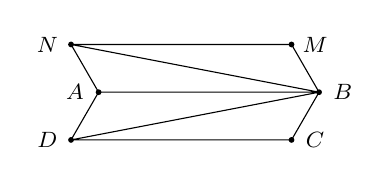
\begin{tikzpicture}[scale=.7, font=\footnotesize, line join=round, line cap=round, >=stealth]
				\path 
				(0,0) coordinate (A)
				(4,0) coordinate (B)
				(A)+(120:1) coordinate (N)
				(A)+(-120:1) coordinate (D)
				(B)+(120:1) coordinate (M)
				(B)+(-120:1) coordinate (C)
				;
				\draw (A)--(B)--(M)--(N)--cycle (A)--(D)--(C)--(B) (N)--(B)--(D);
				\foreach \p/\r in {A/180,B/0,N/180,D/180,M/0,C/0}
				\fill (\p) circle (1.5pt) node[shift={(\r:3mm)}]{$\p$};
			\end{tikzpicture}
		}
		$BD$ có một điểm chung duy nhất $B$ với $(ABMN)$, suy ra $BD$ cắt $(ABMN)$ tại $B$.\\
		$BN$ có hai điểm chung $B$ và $N$ với $(ABMN)$, suy ra $BN\subset (ABMN)$.
	}
\end{ex}
\begin{ex}%[1H4H3-2]%[Dự án dề cương 3 Khối NH24-25-Đợt 3-Võ Thị Thùy Trang]
	\immini[thm]{Cho $E$ và $F$ lần lượt là trung điểm các cạnh $AB$ và $AC$ của tứ diện $ABCD$. Xác định vị trí tương đối của các đường thẳng $BC$, $AD$ và $EF$ với mặt phẳng $(BCD)$.}{
		\begin{tikzpicture}[scale=1, font=\footnotesize, line join=round, line cap=round, >=stealth]
			\path 
			(0,0) coordinate (B)
			(4,0) coordinate (D)
			(2,-1) coordinate (C)
			(B)+(2.5,3) coordinate (A)
			($(B)!.5!(A)$) coordinate (E)
			($(C)!.5!(A)$) coordinate (F)
			;
			\draw (A)--(B)--(C)--(D)--cycle (A)--(C) (E)--(F);
			\draw[dashed] (B)--(D);
			\foreach \p/\r in {A/90,B/180,D/0,C/-90,E/180,F/0}
			\fill (\p) circle (1.5pt) node[shift={(\r:3mm)}]{$\p$};
		\end{tikzpicture}
	}
	\loigiai{
		\begin{itemize}
			\item $BC$ có hai điểm chung $B$ và $C$ với $(BCD)$, suy ra $BC\subset (BCD)$.
			\item $AD$ có một điểm chung duy nhất $D$ với $(BCD)$, suy ra $AD$ cắt $(BCD)$ tại $D$.
			\item $EF$ là đường trung bình của tam giác $ABC$ suy ra $EF\parallel BC$.\\
			$\heva{&EF\parallel BC\\&EF\not\subset (BCD)\\&BC\subset (BCD)}\Rightarrow EF\parallel (BCD)$.
		\end{itemize}
	}
\end{ex}
\begin{ex}%[1H4H3-2]%[Dự án dề cương 3 Khối NH24-25-Đợt 3-Võ Thị Thùy Trang]
	\immini{Cho hai điểm $A$, $B$ cùng thuộc mặt phẳng $(P)$ và một điểm $C$ không thuộc $(P)$. Vẽ đường thẳng $d_1$ đi qua $A$, $B$; $d_2$ đi qua $A$, $C$; $d_3$ đi qua $C$ và song song với $AB$ (hình bên). Tìm số điểm chung của mỗi đường thẳng vừa vẽ với $(P)$. Xét vị trí tương đối của mặt phẳng $(P)$ lần lượt đối với đường thẳng $d_1$, $d_2$, $d_3$.}{
		\begin{tikzpicture}[scale=1, font=\footnotesize, line join=round, line cap=round, >=stealth]
			\path
			(0,0) coordinate (A)
			(4,0) coordinate (B)
			(1,2) coordinate (D)
			($(B)+(D)-(A)$) coordinate (C)
			(2,3) coordinate (E)
			(3,-1) coordinate (F)
			(intersection of E--F and C--A) coordinate (M)
			(intersection of M--F and A--B) coordinate (N)
			(5,2.3) coordinate (G)
			(1,2.3) coordinate (H)
			(intersection of G--H and E--F) coordinate (K)
			;
			\draw (M)--+(0:1.8) (M)--+(180:1) node[above]{$d_1$};
			\draw[fill=black] 
			(M) node[above right]{$A$} circle (1pt) 
			(K) node[above right]{$C$} circle (1pt) 
			($(M)+(0:1.5)$) node[above]{$B$} circle (1pt)
			;
			\draw[dashed] (M)--(N);
			\draw($(F)!0.1!(M)$)node[above right]{$d_2$} (A)--(B)--(C)--(D)--cycle (E)--(M) (N)--(F) (G)--(H) ($(G)!.2!(H)$)node[above]{$d_3$};
			\draw    pic["$P$", draw=black, angle eccentricity=.7, angle radius=1cm]
			{angle=B--A--D}; %góc
		\end{tikzpicture}
	}
	\loigiai{
		Đường thẳng $d_1$ chứa hai điểm $A$, $B$ thuộc $(P)$, vậy $d_1\subset (P)$.\\
		Đường thẳng $d_2$ không nằm trong $(P)$ vì có chứa điểm $C$ không thuộc $(P)$. Mặt khác, $d_2$ lại có điểm $A$ chung với $(P)$, suy ra $d_2$ cắt $(P)$ tại $A$.\\
		$\heva{&d_3\not\subset (P)\\&d_1\subset (P)\\&d_1\parallel d_3}\Rightarrow d_3\parallel (P)$.
	}
\end{ex}
\begin{ex}%[1H4H3-2]%[Dự án dề cương 3 Khối NH24-25-Đợt 3-Võ Thị Thùy Trang]
	\immini[thm]{Cho hình chóp $S.ABC$ có $A'$, $B'$, $C'$ lần lượt là trung điểm của $SA$, $SB$, $SC$. Tìm các đường thẳng lần lượt nằm trong, cắt, song song với mặt phẳng $(ABC)$.}{
		\begin{tikzpicture}[scale=1, font=\footnotesize, line join=round, line cap=round, >=stealth]
			\path 
			(0,0) coordinate (A)
			(4,0) coordinate (C)
			(2,-1) coordinate (B)
			(A)+(2.5,3) coordinate (S)
			($(S)!.5!(A)$) coordinate (A')
			($(S)!.5!(B)$) coordinate (B')
			($(S)!.5!(C)$) coordinate (C')
			;
			\draw (S)--(A)--(B)--(C)--cycle (S)--(B);
			\draw[dashed] (A)--(C);
			\foreach \p/\r in {S/90,A/180,C/0,B/-90,A'/180,C'/0,B'/-45}
			\fill (\p) circle (1.5pt) node[shift={(\r:3mm)}]{$\p$};
		\end{tikzpicture}
	}
	\loigiai{
		\begin{itemize}
			\item $SA$, $SB$, $SC$ là các đường thẳng cắt mặt phẳng $(ABC)$.
			\item $AB$, $BC$, $AC$ là các đường thẳng nằm trong mặt phẳng $(ABC)$.
			\item $A'B'$, $B'C'$, $A'C'$ là các đường thẳng song song với mặt phẳng $(ABC)$.
		\end{itemize}
	}
\end{ex}
	\begin{ex}[Trích đề thi học kì 1 - THPT Ngô Gia Tự - Phú Yên - Năm học 2024-2025]%[1H4H3-3]%[Dự án dề cương 3 Khối NH24-25-Đợt 3-Võ Thị Thùy Trang]
	Cho hình chóp $S.ABCD$ có đáy $ABCD$ là hình bình hành. Gọi $N$, $K$ lần lượt là trung điểm $CD$ và $SB$. Chứng minh rằng $AB \parallel (SCD)$ và $NK\parallel (SAD)$.
	\loigiai{
		\immini{Ta có $\heva{&AB\parallel CD\\&AB\not\subset (SCD)\\&CD\subset(SCD)}\Rightarrow AB\parallel(SCD)$.\\
			Gọi $M$ là trung điểm $AB$.\\
			Ta có $MK$ là đường trung bình của tam giác $SAB$ nên $MK\parallel SA$.\\
			$\heva{&MN\parallel AD\\&MK\parallel SA\\&MN\cap MK=M\\&SA\cap AD=a}\Rightarrow (MNK)\parallel (SAD)$.\\
		Mà $NK \subset (MNK)$ nên $NK\parallel (SAD)$.}
		{	\begin{tikzpicture}[scale=0.8, transform shape]
				\coordinate (D) at (0,0);
				\coordinate (C) at (4,0);
				\coordinate (B) at (5,2);
				\coordinate (A) at (1,2);
				
				\draw[dashed] (A) -- (D);
				
				\coordinate (S) at (0,5);
				\draw (S) -- (B)--(C)--(D)--(S)--(C);
				\draw[dashed] (S) -- (A)--(B) (A)--(D);
				
				
				\coordinate (N) at ($ (C)!0.5!(D) $); % Trung điểm CD
				\coordinate (K) at ($ (S)!0.5!(B) $); % Trung điểm SB
				\coordinate (M) at ($ (A)!0.5!(B) $); % Trung điểm AB
				\coordinate (P) at ($ (S)!0.5!(C) $); % Trung điểm SC
				\draw[dashed](N) -- (K)--(M)--(N);
				\draw (K) -- (P)--(N);
				
				\node[left] at (A) {$A$};
				\node[below right] at (B) {$B$};
				\node[right] at (C) {$C$};
				\node[above left] at (D) {$D$};
				\node[above] at (S) {$S$};
				\node[above] at (K) {$K$};
				\node[below] at (N) {$N$};
				\node[above right] at (M) {$M$};
				\node[left] at (P) {$P$};
		\end{tikzpicture}}
	}
\end{ex}
\begin{ex}[Trích đề thi học kì 1 - THPT Văn Bàn 1 - Tỉnh Lào Cai - Năm học 2024-2025]%[1H4H3-3]%[Dự án dề cương 3 Khối NH24-25-Đợt 3-Võ Thị Thùy Trang]
	Cho hình chóp $S.ABCD$ có đáy $ABCD$ là hình thang với $AD \parallel CB$. Gọi $M$, $N$, $P$ lần lượt là trung điểm của cạnh $SA$, $SB$, $SC$.
	\begin{enumerate}
		\item Chứng minh $NP \parallel (ABCD)$.
		\item Tìm giao tuyến của hai mặt phẳng $(MNP)$ và $(SAD)$.
	\end{enumerate}
	\loigiai{
		\begin{center}
			\begin{tikzpicture}[scale=1, font=\footnotesize, line join=round, line cap=round, >=stealth]
				\path (0,0)coordinate(A)
				--++(1.5,-2) coordinate(B)
				--++(3,0) coordinate(C)
				(A)--+(6,0) coordinate (D)
				--+(0,4) coordinate (S);
				\path (S)--(A) coordinate[midway](M);
				\path (S)--(B) coordinate[midway](N);
				\path (S)--(C) coordinate[midway](P);
				\path (S)--(D) coordinate[midway](Q);
				\draw (M)--(N);
				\draw (N)--(P);
				\draw[dashed] (M)--(P);
				\draw[dashed] (M)--(Q);
				\draw ($(Q)!-0.3!(M)$)node[above]{$x$}--(Q);
				\draw (S)--(B)--(C)--(D)--cycle (S)--(C) (S)--(A) (A)--(B);
				\draw[dashed]  (A)--(D);
				\foreach \p/\q in {A/180,B/-90,C/-90,D/0,S/90,M/180,N/220,P/0}{
					\path (\p) node[shift={(\q:3mm)}]{$\p$};
					\fill[black] (\p) circle (1.2pt);}
			\end{tikzpicture}
		\end{center}
		\begin{enumerate}
			\item Ta có $NP$ là đường trung bình $\triangle SBC$ nên $NP \parallel BC$. \\
			$\heva{&NP \parallel BC\\&BC \subset (ABCD)\\&NP \not\subset (ABCD)}\Rightarrow NP \parallel (ABCD)$.
			\item
			Ta có $\heva{&M\in (MNP)\cap (SAD)\\&NP\parallel AD\\&NP\subset (MNP)\\&AD\subset (SAD)}\Rightarrow (MNP)\cap (SAD)=Mx\parallel AD$.
		\end{enumerate}
	}
\end{ex}
\begin{ex}%[1H4H3-2]%[Dự án dề cương 3 Khối NH24-25-Đợt 3-Võ Thị Thùy Trang]
	Cho hình chóp $S.ABCD$, đáy $ABCD$ là hình bình hành có $O$ là giao điểm hai đường chéo. Cho $M$ là trung điểm của $SC$.
	\begin{enumerate}
		\item Chứng minh đường thẳng $OM$ song song với hai mặt phẳng $(SAD)$ và $(SBA)$.
		\item Tìm giao tuyến của hai mặt phẳng $(OMD)$ và $(SAD)$.
	\end{enumerate}
	\loigiai{
		\immini{\begin{enumerate}
				\item Do $OM$ là đường trung bình của $\triangle SAC$ nên $OM\parallel SA$.\\
				$\heva{&OM \parallel SA\\&SA \subset (SAD)\\&OM \not\subset (SAD)}\Rightarrow OM \parallel (SAD)$.\\
					$\heva{&OM \parallel SA\\&SA \subset (SAB)\\&OM \not\subset (SAB)}\Rightarrow OM \parallel (SAB)$.\\
				\item 
			\end{enumerate}
		}
		{
			\begin{tikzpicture}[scale=1, font=\footnotesize, line join=round, line cap=round, >=stealth]
				\path 
				(0,0) coordinate (A)
				(-2,-1) coordinate (B)
				(4,0) coordinate (D)
				($(B)+(D)-(A)$) coordinate (C)
				(A)+(1,4) coordinate (S)
				($(A)!.5!(C)$) coordinate (O)
				($(S)!.5!(C)$) coordinate (M)
				;
				\draw (S)--(B)--(C)--(D)--cycle (S)--(C) (M)--(D);
				\draw[dashed] (S)--(A) (B)--(A)--(D) (A)--(C) (B)--(D) (O)--(M);
				\foreach \p/\r in {A/135,B/180,C/-45,D/45,O/-90,M/0,S/90}
				\fill (\p) circle (1.5pt) node[shift={(\r:3mm)}]{$\p$};
			\end{tikzpicture}}
		Ta có $\heva{&D\in (OMD)\cap (SAD)\\&OM\parallel SA\\&SA \not\subset (SAD)\\&OM \subset (OMD)}\Rightarrow (OMD)\cap (SAD)=Dx\parallel SA$.
	}
\end{ex}
\begin{ex}%[1H4H3-2]%[Dự án dề cương 3 Khối NH24-25-Đợt 3-Võ Thị Thùy Trang]
	Cho hai hình bình hành $ABCD$ và $ABEF$ không nằm trong cùng một mặt phẳng. Gọi $O$ và $O'$ lần lượt là tâm của $ABCD$ và $ABEF$.
	\begin{enumerate}
		\item Chứng minh đường thẳng $OO'$ song song với các mặt phẳng $(CDEF)$, $(ADF)$ và $(BCE)$.
		\item Gọi $M$ và $N$ lần lượt là trung điểm của $AF$ và $BE$. Chứng minh $MN\parallel (CDFE)$.
		\item Tìm giao tuyến của hai mặt phẳng $(OMN)$ và $(ABCD)$.
	\end{enumerate}
	\loigiai{
		\begin{enumerate}
			\item 
			\immini{\begin{itemize}
					\item Ta có $OO'$ là đường trung bình của tam giác $ACE$, suy ra $OO'\parallel CE$.\\
					Khi đó, $OO'$ không nằm trong mặt phẳng $(CDEF)$ và $OO'$ song song với $CE$ nằm trong $(CDEF)$, suy ra $OO'\parallel (CDEF)$.
					\item Ta có $OO'$ không nằm trong mặt phẳng $(BCE)$ và $OO'$ song song với $CE$ nằm trong $(BCE)$, suy ra \break $OO'\parallel (BCE)$.
					\item Ta có $OO'$ là đường trung bình của tam giác $BDF$, suy ra $OO'\parallel DF$.\\
					Khi đó, $OO'$ không nằm trong $(ADF)$ và $OO'$ song song với $DF$ nằm trong $(ADF)$, suy ra $OO'\parallel (ADF)$.
			\end{itemize}}{
				\begin{tikzpicture}[scale=1, font=\footnotesize, line join=round, line cap=round, >=stealth]
					\path 
					(0,0) coordinate (A)
					(0,-3) coordinate (B)
					(-1.5,-2) coordinate (C)
					($(A)+(C)-(B)$) coordinate (D)
					(2,-2) coordinate (E)
					($(A)+(E)-(B)$) coordinate (F)
					($(A)!.5!(C)$) coordinate (O)
					($(A)!.5!(E)$) coordinate (O')
					($(A)!.5!(F)$) coordinate (M)
					($(B)!.5!(E)$) coordinate (N)
					;
					\draw (A)--(D)--(C)--(B)--(E)--(F)--cycle (A)--(B) (M)--(N) (A)--(C) (A)--(E) (D)--(F);
					\draw[dashed] (N)--(O)--(M) (C)--(E) (O)--(O');
					\foreach \p/\r in {A/90,B/-90,O/180,O'/0,D/135,C/-135,E/-45,F/45,M/90,N/-90}
					\fill (\p) circle (1.5pt) node[shift={(\r:3mm)}]{$\p$};
				\end{tikzpicture}
			}
			\item Do $ABEF$ là hình bình hành suy ra $MN\parallel EF$ (do $M$, $N$ lần lượt là trung điểm của $AF$, $BE$).\\
			Ta có $MN$ không nằm trong $(CDEF)$ và $MN$ song song với $EF$ nằm trong $(CDEF)$, suy ra $MN\parallel (CDEF)$.
			\item Do $ABEF$ là hình bình hành suy ra $MN\parallel AB$ (do $M$, $N$ lần lượt là trung điểm của $AF$, $BE$).\\
			Mà hai mặt phẳng $(OMN)$ và $(ABCD)$ có điểm chung là $O$ và đi qua hai đường thẳng song song $MN$ và $AB$.\\
			Suy ra giao tuyến của hai mặt phẳng $(OMN)$ và $(ABCD)$ là đường thẳng $d$ qua $O$ và song song với $MN$.
		\end{enumerate}
	}
\end{ex}
\begin{ex}[Trích đề thi học kì 1 - THPT Thị Xã Quảng Trị - Năm học 2024-2025]%[1H4H3-2]%[Dự án dề cương 3 Khối NH24-25-Đợt 3-Võ Thị Thùy Trang]
	Cho hình chóp $S.ABCD$ có đáy $ABCD$ là hình thang thỏa mãn $AB\parallel CD$ và $AB=2CD$. Gọi $H$ là điểm thuộc cạnh $SD$ sao cho $\dfrac{SH}{SD}=\dfrac{2}{3}$. Chứng minh $SB \parallel (AHC)$.
	\loigiai
	{\immini
		{Trong mặt phẳng $(ABCD)$, gọi $O$ là giao điểm của $AC$ và $BD$.\\
			Vì $AB\parallel CD$ nên hai tam giác $OAB$ và $OCD$ đồng dạng, do đó
			$$\dfrac{OD}{OB} = \dfrac{DC}{AB} = \dfrac{DC}{2DC} = \dfrac{1}{2} \Rightarrow \dfrac{DO}{DB} = \dfrac{1}{3}.$$
			Xét tam giác $DSB$, có $H$, $O$ lần lượt thuộc các cạnh $DS$ và $DB$. Ta có $\dfrac{DO}{DB} = \dfrac{DH}{DS} = \dfrac{1}{3}$ nên $HO \parallel SB$.\\
			Mặt khác $SB$ không nằm trong mặt phẳng $(AHC)$, $HO \subset (AHC)$ nên $SB \parallel (AHC)$.}
		{\begin{tikzpicture}[scale=0.9, font=\footnotesize,line join=round, line cap=round, >=stealth]
				\def\h{3}
				\path (0,0) coordinate (A)
				(-1.6,-1.2) coordinate (D)
				++(3,0) coordinate (C)
				($(A)+2*(C)-2*(D)$) coordinate(B)
				(intersection of A--C and B--D) coordinate(O)
				(0.5,\h) coordinate(S)
				($(S)!2/3!(D)$) coordinate(H);
				\draw (S)--(B)--(C)--(D)--(S)--(C)--(H);
				\draw[dashed] (S)--(A)--(B)--(D)--(A)--(C) (A)--(H)--(O);
				\foreach \diem/\pos in {A/40, B/-90, C/-90, D/-90, S/90, H/170, O/90} \fill (\diem) node[shift={(\pos:0.3)}] {$\diem$} circle(1pt);
	\end{tikzpicture}}}
\end{ex}















